\chapter*{Appendix}
\addcontentsline{toc}{chapter}{Appendix}
\section*{List of appendices}
\vspace{-8em}
\listofanhang
\clearpage
\spezialkopfzeile{Appendix} % damit in der Kopfzeile das Wort "Anhang" angezeigt wird


\anhang{Requirements elicitation} \label{anhang:ReqEng}

The requirements gathering process for this research, presented in chapter \ref{chap:ReqEng} follows closely the requirements elicitation activity, which is an activity of requirements engineering in software engineering. Requirements engineering is a set of activities to develop, document, and manage the specifications a system is expected to meet.\footcites[Cf.][p.16]{SommervilleIntegratedrequirementsengineering2005}[cf.][p.38]{PatakiSystemRequirementsAnalysis2003}

Firstly, it is important to clearly understand what requirements are: Requirements are descriptors of what a system should do, defining services the ideal system must provide and the constraints under which the system must operate.\footcites[Cf.][p.100]{SommervilleSoftwareengineering2011}[cf.][p.95]{IEEEIEEEstandardglossary1990} Requirements can range from high-level abstract statements of services or system constraints to very detailed functional specifications\footcite[Cf.][p.215]{DavisSoftwarerequirementsobjects1993} and may be divided into functional requirements and non-functional requirements, described in the list below.

\begin{itemize}
    \item \textbf{Functional requirements} A functional requirement defines a function the system must perform.\footcite[Cf.][p.34]{IEEEIEEEstandardglossary1990} It specifies how the system should react to particular inputs and how the system should behave in specific situations.\footcite[Cf.][p.102]{SommervilleSoftwareengineering2011} It defines what actions the system must do (functionality) rather than how it performs these actions. 
    \item \textbf{Non-functional requirements} A non-functional requirement refers to additional requirements which put constraints on the functionality. These constraints may be a consequence of product requirements, organizational policies or external factors (e.g. reliability, standard processes, interoperability) and often apply to the whole system rather than individual features.\footcite[Cf.][p.102]{SommervilleSoftwareengineering2011}
\end{itemize}

Separating the requirements gathering from the design process helps to find an objective solution, because the solution is not influenced by design considerations and the requirements do not limit the implementation of the system. The requirements elicitation is the first activity of the requirements engineering process, as presented in figure \ref{fig:REAll}.\footcites[Cf.][p.116]{SommervilleSoftwareengineering2011}[cf.][pp.17]{SommervilleIntegratedrequirementsengineering2005} 

These requirements are collected during the requirements elicitation phase, which is the first of a set of activities in requirements engineering.\footcites[Cf.][p.116]{SommervilleSoftwareengineering2011}[cf.][p.17]{SommervilleIntegratedrequirementsengineering2005} The requirements engineering process is somewhat ill-defined, with different authors presenting different activities and practitioners using a large number of different methods to develop the requirements.\footcite[Cf.][p.225]{ZhangEffectiverequirementsdevelopmentA2007} The main aspects of the requirements engineering process is visualized in figure \ref{fig:REAll}. The process starts with the elicitation of the requirements from a variety of knowledge sources in order to collect needed information. The requirements are consequently analyzed in order to detect overlaps and conflicts and the generated knowledge is then added to the understood knowledge.\footcite[Cf.][p.17]{SommervilleIntegratedrequirementsengineering2005} That understood knowledge serves as input for the next step, the specification, where the requirements are structured and recorded in a document (the structured requirements specification (SRS)). The documentation may be done via natural language or dedicated conceptual models, so that the requirements are clear, understandable and correct, and constitutes the final output of the overall requirements engineering process.\footcites[Cf.][p.17]{SommervilleIntegratedrequirementsengineering2005}[chapter 1]{PohlRequirementsengineeringfundamentals2011} The fourth activity comprises the validation of these requirements. It checks again if the requirements are correct and that they indeed correspond to the stakeholders' needs.\footcite[Cf.][p.17]{SommervilleIntegratedrequirementsengineering2005}
It is an iterative cycle, as inconsistent, ambiguous or missing information that is uncovered during the specification or validation steps is tried to be resolved in another elicitation session. 
Major players in the literature agree on these four main activities,\footcites[Cf.][p.225]{ZhangEffectiverequirementsdevelopmentA2007}[cf.][p.220]{DavisSoftwarerequirementsobjects1993}[cf.][chapter 1]{PohlRequirementsengineeringfundamentals2011}[cf.][p.116]{SommervilleSoftwareengineering2011} but Sommerville and Pohl and Rupp also add negotiation (reconciling conflicting stakeholders' views) and management (actively controlling the changes to the requirements) to create a full picture of the requirements engineering process.\footcites[Cf.][p.17]{SommervilleSoftwareengineering2011}[cf.][chapter 1]{PohlRequirementsengineeringfundamentals2011}

\begin{figure}
    \centering
    \includesvg[width=\textwidth]{graphics/Zhang_textcurves}
    \caption[Summary of the requirements engineering process.]{Summary of the requirements engineering process.\footnote{With changes taken from \cite{ZhangEffectiverequirementsdevelopmentA2007}, p.225.}}
    \label{fig:REAll}
\end{figure}
%\footnotetext{With changes taken from \cite{ZhangEffectiverequirementsdevelopmentA2007}, p.225}
Since this research bases the requirements gathering on the requirements elicitation activity, only this activity and the methods used for its execution are more closely examined in the following paragraph. 

\paragraph{Requirements Elicitation} Requirements elicitation refers to the gathering of information to extract the requirements that the system has to fulfill. Possible sources of information that allow the discovery of requirements need to be identified.\footcites[Cf.][p.2]{TiwariMethodologySelectionRequirement2017}[cf.][p.17]{SommervilleIntegratedrequirementsengineering2005} These knowledge sources may be the stakeholders (users, project sponsors, managers) as presented in figure \ref{fig:REAll}, or other resources (e.g. existing systems). It is important to not only discover but to fully understand the needs of these potential stakeholders in order to communicate them to the system developers. Therefore, the elicitation of the requirements is an important and critical step in the RE process and requires the use of appropriate methods.\footcites[Cf.][p.232]{ZhangEffectiverequirementsdevelopmentA2007}[cf.][pp.19 et seq]{ZowghiRequirementselicitationsurvey2005}

The gathering of information, and subsequently of the requirements may be done in numerous ways. These methods may be categorized by their common nature:\footcite[Cf.][p.170]{HickeyElicitationtechniqueselection2003} 
\begin{itemize}
    \item \textbf{Conversational methods}: Interview, questionnaire, survey\footcites[Cf.][chapter 3]{PohlRequirementsengineeringfundamentals2011}[cf.][p.170]{HickeyElicitationtechniqueselection2003}
    \item \textbf{Observational methods}: Social analysis, observation, ethnographic study\footcites[Cf.][p.227]{ZhangEffectiverequirementsdevelopmentA2007}[cf.][p.173]{HickeyElicitationtechniqueselection2003}
    \item \textbf{Creative methods}: Brainstorming, analogy techniques\footcite[Cf.][chapter 3]{PohlRequirementsengineeringfundamentals2011}
    \item \textbf{Analytic methods}: Requirement reuse, documentation study, protocol analysis, discourse analysis \footcites[Cf.][p.12]{GoguenTechniquesrequirementelicitation1993}[cf.][pp.227-228]{ZhangEffectiverequirementsdevelopmentA2007}[cf.][p.2]{TiwariMethodologySelectionRequirement2017}
    \item \textbf{Synthetic methods}: Scenarios, prototyping, joint application development, perspective based reading\footcites[Cf.][p.228]{ZhangEffectiverequirementsdevelopmentA2007}[cf.][chapter 3]{PohlRequirementsengineeringfundamentals2011}[cf.][p.3]{TiwariMethodologySelectionRequirement2017}
\end{itemize}

The observational methods put the researchers in a more passive role, where they observe the stakeholders in a certain situation and notes the work process, potential mistakes, risks, and open questions, which constitute the inputs for the formulation of the requirements.\footcite[Cf.][chapter 3]{PohlRequirementsengineeringfundamentals2011} Creative methods, as the name suggest, serve the purpose to discover new and innovative requirements.\footcite[Cf.][chapter 3]{PohlRequirementsengineeringfundamentals2011} Analytic methods focus on extracting requirements from existing documents, making them especially useful to quickly formulate fine-grained requirements from existing documentation.\footcite[Cf.][p.228]{ZhangEffectiverequirementsdevelopmentA2007} Finally, synthetic methods are a combination of conversational, observational, creative, and analytic techniques.\footcite[Cf.][p.228]{ZhangEffectiverequirementsdevelopmentA2007} 

All techniques and methods have their strengths and weaknesses, which is why a combination of methods is often used in practice. Nonetheless, conversational methods have proven to be the primary method to effectively collect knowledge, because they provide a natural way to express ideas, problems, and questions.\footcites[Cf.][pp.226/227]{ZhangEffectiverequirementsdevelopmentA2007}[cf.][p.42]{ZowghiRequirementselicitationsurvey2005}


\anhang{Detailed question compendium}

\newcolumntype{P}[1]{>{\centering\arraybackslash}p{#1}}
\captionsetup{list=no}
\begin{table}[H]
		\begin{tabular}{ | p{0.7cm} P{2.6cm} p{5cm} p{6cm}|}
		\hline
	No. & Question & Expected Answer & Further questions \\ \hline
	1a & What is your role within HPE? & Description of their work; daily business; their tasks. "I am … and my overall task is to …. For this, I do … and …" & Could you please elaborate on this further? What exactly do you <sell/do>? \\ \hline
	1b & Who are your clients?  & Description of their business partners, their industry, the level of their partners (CIO, Managers. Developers, …). "I work with…" & From what industry do most of your clients come? What region are they from? For what purpose do they come to you? What problems drive them? \\ \hline \hline
	2a & What do you understand under the term "blockchain"?  & Short definition of the blockchain technology. "Blockchain is a data structure, which allows the secure and immutable storage of data, …" & Is the term familiar to you? Where did you first hear about it? In which context? \\ \hline
	2b & How did you gain an understanding of blockchain?  & Description of learning resources used to get to know blockchain. "I watched a lot of YouTube videos" or "I talked with my colleagues" or "I read books about it" etc. & How much time did you spend on trying to learn about the technology? How did you do this? How many resources did you look at? \\ \hline
	2c & Many find it hard to understand this topic. In your opinion, what might be the cause for this?  & Description of the different reasons why blockchain is difficult. "It's complex", "Many different underlying concepts", "Takes too long", … & Did you have any trouble understanding this topic? Why do you think so? Which topic do you find very difficult to understand? \\ \hline
	2d & What do you think is the best way to learn about this new technology?  & Short brainstorming and presentation of various learning resources. "Learning works best with examples" or "I would recommend …." & In general, how do you learn best? What would you consider a good way to learn about technical concepts? What platforms do you recommend?  \\ \hline
	2e & Why might blockchain be interesting to you or your clients? What improvements do you expect?  & Description of use cases specific to their role or industry. "I think it might be used in …" or "I think it would help my clients do …" & What do you think are general use cases for blockchain? How can HPE attribute to this? \\\hline
    \end{tabular}
    \caption{Detailed question compendium for the expert interviews, questions 1a to 2e}
    \label{tab:my_label}
\end{table}

\begin{table}[H]
    \centering
    \begin{tabular}{ | p{0.7cm} P{2.6cm} p{5cm} p{6cm}|}
    \hline
    2f & How would you estimate your clients’ knowledge about blockchain? & Brief estimation of what their clients know of blockchain. "I think they know …" or "They probably don't know anything" & Could you give an estimate on their competency regarding blockchain? On which level do you think they know this topic? \\\hline
    2g & What is your opinion regarding the current hype about blockchain? & Commentary to the blockchain hype, maybe because of the price surge or the media coverage. "I feel it is just hot air" or "I feel that behind the hype there is some truth .." & What is for you "hype"? Would blockchain fall under this issue? From where do these hype-issues originate? Do you think blockchain will live up to its name? \\ \hline \hline
	3a & What do you think is the optimal way to explain blockchain to novices?  & Short brainstorming and presentation of various learning resources and estimation of abstraction level of an appropriate explanation. "It should start with …" & How would you explain blockchain to your peers? What concepts would you include? Which ones not and why? \\ \hline 
	3b & What components of a blockchain should it contain? & Enumeration of the most important concepts of blockchain technology. "Hash values" or "immutable ledger" or "cryptography", etc. & What is the most important aspect of blockchain? What concepts is it based on? \\ \hline
	3c & How should such an explanation be structured to be helpful for clients? What additional information should it include?  & Brainstorming how the explanation would change for a business context. "It should show which problem it solves by …" or "More relevant examples" & What interests your clients/partners in a technology? What are they looking for in a technology? What do they expect to receive from it? \\ \hline
    \end{tabular}
    \caption{Detailed question compendium for the expert interviews, questions 2f to 3c }
    \label{tab:my_label}
\end{table}


\anhang{Interview Transcripts}\label{Interviews}

\lstset{language=TeX, % hervorzuhebende Keywords definieren
  morekeywords={anhang, anhangteil}
}


% Um den Anforderungen der Zitierrichtlinien nachzukommen, wird das Paket \verb|tocloft| verwendet. Jeder Anhang wird mit dem (neu definierten) Befehl \lstinline|\anhang{Bezeichnung}| begonnen, der insbesondere dafür sorgt, dass ein Eintrag im Anhangsverzeichnis erzeugt wird. Manchmal ist es wünschenswert, auch einen Anhang noch weiter zu unterteilen. Hierfür wurde der Befehl \lstinline|\anhangteil{Bezeichnung}| definiert.

% In~\ref{anhang:abbildung} finden Sie eine bekannte Abbildung und etwas Source Code in~\ref{anhang:sourcecode}. 

\anhangteil{Interview with Daniel Kaltenbach}\label{anhang:InterviewDK}
This is the transcription of the complete interview between Daniel Kaltenbach (Interviewee, DK) and the author (Interviewer, LM). The interview was conducted on 22th of March, 2018 from 9:00 to 9:30 in person in the HPE office in Böblingen. 

\begin{xlist}
     \item[LM] Ok, jetzt haben wir das Interview gestartet. Noch eine Sache ganz vorweg, ist es okay, wenn ich deinen Namen in der Bachelorarbeit nenne oder möchtest du es lieber anonym machen?
     \item[DK] Lass uns das am Ende klären.
     \item[LM] Das war immer so am Anfang, also bei den Ausführungen in den Büchern ist immer noch: Ja, das muss man einmal festhalten. Aber erstmal etwas über dich! Was ist denn deine Rolle in HPE?
     \item[DK] Ja, also mein Name for the record. Ich heiße Daniel Kaltenbach und bin bei HPE verantwortlich für das Thema IOT. Ich bin für Deutschland, Österreich und Schweiz sowie in Russland der designierte IOT-Verantwortliche, der eben die Kooperationsstrategie dieses Themas vorantreibt und eine cross-funktionale Inkubationsorganisation führt um das Thema IOT für HPE greifbar zu machen, Portfolio, Partnerschaften und strategische Initiativen zu treiben, zu verantworten und nachher zu Marktkapitalisierung führen zu lassen.
     \item[LM] Ok, und wer zählt so zu deinen Kunden? Oder hast du direkt Kontakt zu Kunden?
     \item[DK] Ich habe ganz viel direkten Kontakt mit Kunden. Ich habe aber keine direkten eigenen Kunden, also ich bin ja kein Account Manager oder so, weil ich vertrete das Thema im Namen der HPE und damit ist mein Kunde die Geographie Deutschland, Österreich, Schweiz und Russland.
     \item[LM] Okay, worauf ich eher damit hinaus wollte, so was was macht ihr denn für eure Kunden? Also welche Angebote und Dienstleistungen von IOT her bietet ihr an?
     \item[DK] Enorm unterschiedlich. Ich nutze ganz gern die Analogie, die die PWC geprägt hat. Wenn sie IOT definieren, dann gibt es im Prinzip intelligente Produkte: Die Kaffeemaschine, die nach Hause telefoniert und weiß, wann sie kaputt gehen wird. Wohlgleich das zweite Thema des intelligenten Prozesses, wo es eben um horizontale Integration von Prozessketten geht, die schlussendlich in der Summe intelligenter werden, oder nicht. Also wenn ich weiß, was eben nach mir passiert, dann kann ich möglicherweise nacharbeiten was davor nicht so gut gelaufen ist. Ich kann die Qualität im Gesamtprozess betrachten, den Durchlauf optimieren. Wenn ich weiß, dass der vor mir fertig ist, kann die nachfolgende Maschine schon einmal anlaufen und sich aufwärmen, weil sie ja gleich einen Prozess bekommen wird et cetera. Das kann aber auch mein Customer Journey sein, der durch ein Retail läuft und eben, wenn jemand rein läuft dann ist es wichtig, dass ein Mitarbeiter hinten weiß, da ist jemand reingelaufen, damit ich ihn möglicherweise richtig ansprechen kann. Solche Dimensionen, also intelligentes Produkt oder intelligenter Prozess und darin beraten wir und liefern jetzt die Technologien, die helfen von diesen Daten, von diesen Informationen, die da sind, Herr zu werden und darauf basierend intelligente Entscheidungen zu treffen.
     \item[LM] Ok dann würde ich jetzt auch schon direkt zum nächsten Teil gehen. Zum Thema: Das Problem beim Verständnis von Blockchain. Ganz allererst: Was verstehst du genau unter Blockchain und was stellst du dir unter der Funktionsweise davon vor?
     \item[DK] Ich stelle mir erstmal vor, dass es etwas unheimlich Kompliziertes ist und ich glaube ich nehme damit teilweise schon die Frage vorweg was das Problem da dran ist. Ich glaube das ist Teil des Problems. Also es ist eine Technologie ja erstmal, die eben ähnlich einer Datenbank funktioniert aber eben dezentral die Daten hält und gegenseitig autorisiert. Das würde ich jetzt mal so wie als eine Blockchain beschreiben, wie eine Art verteiltes Dateisystem, verteiltes Datenbanksystem, das eben aber ein in sich, durch die Verteilung notwendiges Problem löst, eben das der Autorisierung der Daten und der Richtigkeit. Wahrscheinlich medium richtig, aber das war jetzt zumindest mein Verständnis davon.
     \item[LM] Das reicht ja auch und wie hast du dir… also woher hast du jetzt dieses Verständnis? Also hast du das von vom Hörensagen, von irgendwelchen Artikeln oder wie hat sich das so zusammen geflochten?
     \item[DK] Mischung von allem. Ich glaube, dass warum es noch so medium richtig ist, liegt daran, dass ich mich einfach nie selbst mit dem Thema intensiv auseinandergesetzt habe und einfach mal wirklich hinter das Thema gestiegen bin und deshalb hier die Arbeit auch ganz gut. Ich glaube das ist was, was die Industrie an der Stelle momentan nicht schafft: Eine sinnvolle Artikulation der Technologie und damit verbunden der Anwendungsszenarien. Also die Übersetzungen von einfachen Menschen, wie mir hin zu „Wir verstehen die Technologie und wir benutzen sie für dich“. Dazu ist mein Wissen nicht ausreichend und das schafft die Industrie auch nicht. Also mein Wissen basiert auf unterschiedlichsten Gesprächen, Konferenzen und ich war durchaus mal bei dem ein oder anderen Blockchain-artigen Workshop, wo durchaus nochmal so Grundlagen waren, aber immer wenn ich es gehört habe war es immer irgendwie nochmal ein bisschen neu und ein bisschen anders. Und einer hatte das so und der andere wieder so und ich bin halt nicht Techniker, ich mache Vertrieb am Ende des Tages.
     \item[LM] Ja das ist auch je nachdem wo man im Internet guckt, gibt es ganz viele verschiedene Ansätze das zu erklären. Ich versuche eben auch einmal die zu konsolidieren und zu schauen, dass man einen Ansatz hat, der das ganzheitlich aber auch relativ einfach erklärt. Und wieso noch einmal meintest du denn, dass du dich eben nicht weiter damit auseinandergesetzt hast? Also du meintest ja so: Ja, es ist ein kompliziertes Thema; Hat dich das einfach davon abgeschreckt oder war es die fehlende Zeit? Was waren so die Gründe, dass du jetzt noch nicht da groß hinter stehst. 
     \item[DK] Zeit und Relevanz. Also wenn ich mich mit jeder Technologie irgendwie auseinandersetzen würde, die irgendwie IOT relevant ist, dann würde ich wahrscheinlich die nächsten zehn Jahre studieren und hätte es dann erst recht nicht gelernt, weil in den zehn Jahren wieder neue Sachen draußen sind. Also ich muss natürlich extrem selektiv wahrnehmen und das tue ich auch. Ich verstehe und das ist glaube ich mehr dieses Hörensagen, dass es eine signifikante Implikation haben kann für bestimmte Anwendungsszenarien. Ich habe bisher für mich noch nicht den Bedarf verspürt mich intensiver damit auseinanderzusetzen, weil immer dann wenn so eine Diskussion aufgekommen wäre oder hätte kommen können, habe ich mir einfach einen Experten dazu geholt. Das bringt meine Rolle glücklicherweise mit, dass ich darin nicht Experte sein muss.
     \item[LM] Ja, du meintest gerade, dass es schon Implikationen für IOT/deinen Bereich hat. Hast du da irgendwelche Beispiele im Kopf, wo du sagen könntest: Ja, Blockchain könnte da und da bedeutend sein? Also eher für deinen Bereich, jetzt nicht auf Finanzderivate bezogen.
     \item[DK] Ja, du wirst jetzt unfair. Nenee, ich glaube es ist ein gute Frage! Ich habe da jetzt natürlich irgendwie 20 Beispiele im Kopf, die irgendwie so allgemein diskutiert werden. Aber wenn ich jetzt so darüber nachdenke, kann ich jetzt nicht mit Bestimmtheit sagen, dass ich weiß, dass dieser Use Case oder dieser Anwendungsfall wirklich idealtypisch für eine Blockchain-Implementierung ist, weil ich auch weiß Blockchain ist nur eine Technologie, ne. Es gibt auch noch mögliche andere Technologien, die möglicherweise diesen Use Case genauso gut oder besser gar bedienen können. Von daher kann ich dir jetzt gerade keinen idealtypischen Fall nennen, weil mir wahrscheinlich auch die Technologie zu unbekannt ist.
     \item[LM] Darauf will ich auch eigentlich gar nicht hinaus, also es soll jetzt nicht DER Use Case sein, wo du denkst, auf jeden Fall muss da Blockchain hin. Sondern es geht auch gerade um dieses Hörensagen, was die meisten anderen Leute so als Use Cases nennen. Ich würde gerne von dir wissen, was du denn so dazu zählst.
     \item[DK] Ja, ähm, alles was natürlich in den Bereich Monetarisierung geht, wo man eben den Mediator ausschalten möchte, also wie eine Bank oder so, wo man ein aufwändiges Transaktionssystem benötigen würde. Wo eben Maschinen mit Maschinen Payments irgendwie ablaufen, würde ich jetzt mal so zu diesen Daten-Monetarisierungsbereich und Maschinen zu Maschinen Payments und natürlich das Thema Smart Contracting in der zweiten Dimension. Wo eben Maschinen miteinander verhandeln und so sich schlussendlich einigen auf Arbeitsausführungen und ja dann das Payment möglicherweise als zusätzliche notwendige Komponente mit einfließen lassen aber nicht notwendigerweise. Das wären jetzt so die zwei schwergewichtigsten. Aber ich bin wahrscheinlich zu weit weg um sagen zu können, das wäre perfekt oder so.
     \item[LM] Das ist ja alles gut und musst du auch gar nicht. Gut, zu der Frage wieso das so schwer zu verstehen ist, haben wir ja schon festgehalten, dass es eben eine komplizierte Technologie ist. Meinst du da gibt es noch andere Punkte, dass sich eben die Leute/die Personen/potenzielle Kunden in deinem Gebiet sich noch nicht so sehr mit dem Thema auseinandergesetzt haben oder dieses Halbwissen haben, woran das liegen könnte?
     \item[DK] Mehrere Antworten. Weiterführend zu dem Thema "komplizierte Technologie" ist glaube ich typischerweise  (und ich glaube das ist in allen Technologien so), wenn wir  beginnen über die Technologie zu sprechen, dann ist das immer ein Technologen-Kreis. Und ein Mensch/ein Typ Mensch, der natürlich hoch technisch ist, wenn der dir versucht nachher, also ich meine dir und mir, ich will dir jetzt nichts unterstellen, aber zumindest mir, der einfache Mensch, dann versucht etwas Kompliziertes zu erklären, dann muss der immer fachlich total richtig sein. Wenn Physiker, der dir gegenüber sitzt und dir die Welt erklärt. Die Welt ist manchmal ganz einfach. Einen Fuss vor den anderen setzen, bewegst dich. Ja das ist für den nicht so einfach, da sind Energie, Bewegungsabläufe, da sind Erdanziehung, schlag mich tot. So ist es hier auch ein bisschen. Ich glaube, es ist noch nicht die Community oder die Technologiegruppe nenne ich sie mal, jetzt mal irgendwie verdreht, dass sie noch nicht in der Lage sind eine einfache Sprache zu finden, als sie sich selbst einfach noch so Technologie-verliebt sind und den Transfer in die einfache Menschenwelt nicht schaffen. Nummer 1, also die Gruppe der Menschen, die damit beschäftigt sind. Die zweite Dimension ist: Wir leben momentan, glaube ich jetzt in so einer Technologiespirale, in der einfach enorm viele Techniken gerade unterwegs sind, die irgendwie alle auf uns einpressen. Sagen wir mal 5G als Kommunikationsstandard, das ist künstliche Intelligenz, 3D Druck, es gibt irgendwie 50 solcher Dinge. Und die Menschen sind in Summe noch in so einer Abwartephase. Welche von den Dingern werden jetzt revolutionsartig meine Welt verändern, mit welchen muss ich mich auseinandersetzen? Das sind so viele, dass wir eine Überforderung haben an Dingen, die die Menschen typischerweise nicht verstehen, weil sie einfach kompliziert sind. Weil das eben die Evolution von Technik ist. Ich glaube, das sind so die zwei Dimensionen. Also, in der Gruppe der Technologen ist man noch nicht bereit eine einfache Sprache zu wählen, weil das technische Thema einfach noch zu technisch ist. Oder man sich aber so sehr die Technik differenziert. Und gleichwohl bewegen wir uns in einem Umfeld, wo Technologien so rapide und so viele da sind und auch wieder weg gehen, dass die Leute sich nicht genug damit auseinandersetzen zu können.
     \item[LM] Vielen Dank. Jetzt zu der nächsten Frage, die war: So wir haben jetzt schon gesagt, ja welche möglichen Konzepte bei IOT für Blockchain gibt es. Denkst du auch, dass das für HPE und die Kunden interessant sein könnte, das mal einzuführen für ein paar Use Cases?
     \item[DK] Technologie ist ein Vehikel. Und Blockchain ist an der Stelle ein Vehikel, weil es eine Datenbank ist, und Technik ist ein Vehikel, die am Ende des Tages Mehrwerte schaffen müssen.  Und für Kunden sind Mehrwerte relevant, wir müssen Business Outcomes mit denen diskutieren, Gründe, Verbesserungen des Produktes, für Qualität, wie waren wir beim Ausbringen und mehr ausbringen, Kosten reduzieren oder ganz klassisch und Wissensfragen und sobald wir es schaffen zu übersetzen, warum Blockchain da einen Beitrag leisten kann oder ein auf Blockchain basierendes Anwendungsszenario, das deswegen komplizierter ist aber Blockchain als ein technologisches Element da drin hat. Dann sind die hoch zufrieden damit und momentan sind wir noch in so einer Phase, wo die Leute geil finden, dass Blockchain da drin ist. Das keinen Mehrwert hat, weil es halt geil ist Blockchain gemacht zu haben. Der Sache wegen geil. Aber ich glaube, das kühlt sich in der nächsten, das dauert gar nicht mehr lange, in den nächsten sechs Monaten wird sich das noch ein bisschen regen und dann wird der Markt da sein, verstanden haben: Okay, ist es ein Werkzeug in einem großen Werkzeugkasten und setzt das ein bitte. Also ihr macht das, ihr löst das IT Problem da. Und Blockchain ist offensichtlich eins der Werkzeuge, sowie beim Handwerker, mir ist dann vollkommen egal ob der einen großen Schraubenzieher oder kleinen hat, so lange die Schraube eingedreht wird. Schraube in der Wand. Im Grunde: Reduktion von Kosten und wenn Blockchain das Thema dafür ist, dann geil machst du das. Aber ich glaube, das ist nicht momentan, sechs Monate noch.
     \item[LM] Glaubst du denn, dass wenn man dem Kunden dann erklärt, wie die Blockchain funktioniert, ob das einen Einfluss darauf hat? Also so wie du es anlauten ließest war es ja eher nicht der Fall. Also dass er sagt, Blockchain für mich egal wie das funktioniert, Hauptsache es funktioniert. Oder denkst du auch, dass er daran interessiert sein könnte zu wissen, wie es funktioniert? 
     \item[DK] Mehrere Stufen. Zuerst interessiert ihn, was ist der Business Outcome. Und natürlich will er irgendwann verstehen, ist dieses Angebot, dass ich von dir bekomme, liebes Technologieunternehmen, hat das Substanz? Wie ist das umgesetzt? Hat das, möglicherweise (weil wir erklären natürlich ihm die Straße nach nirgendwo oder zu seinem Business Problem). Aber er hat ein Ökosystem, in das er es einbetten muss. In ein Business Continuity System, das heißt er muss verstehen was passiert, wenn diese Lösung oder diese Technik von dir ausfällt. Gibt es ein Backup und Disasterplan, was wollen wir nicht. Und wir werden in diesem Angebot, in dieser Erstdiskussion, werden wir natürlich alle Aspekte erläutern. Das heißt in dem Moment, wo er eben tiefer einsteigen möchte oder wo wir bewiesen haben, ja wir können ihr technisches Problem lösen mit Technologie. Würde er fragen: Welche Technologie verwendest du und was sind dafür die Disasterprozesse? Was denn, wie sicher ist das? Ist die Technik morgen weg? Also gibt es ein Substitut? Was auch immer, da wird es sicherlich eine Diskussion geben und dann ist die Technik wichtig, wenn dann die Technologie Blockchain eine entsprechende Kredibilität erreicht, die ihm nützt, dann absolut. Es gibt Technologien von der wir heute sagen würden, wir machen den Prozess und der Kunde guckt dahinter und du würdest sagen: Und ich liefere Ihnen dann eine DVD. Dann würde er tot umfallen. Wahrscheinlich wenn ich eine Kassette noch liefern würde, noch zweimal tot umfallen und sagen: Ihr seid kein kredibles Unternehmen, weill sie keine Technologien nehmen, die nicht mehr State of the art ist, und eben kein zukünftiges ordentliches Substitut mehr hat oder keine Wiedersupply hat. Von daher hat es da sicherlich eine Relevanz, wenn sich die Technik durch setzt, aber die Technologie alleine macht keinen Mehrwert.
     \item[LM] Ja, da stimme ich auch zu. Mhmm und woran meinst du liegt es, dass Blockchain momentan so ein Hype ist? Beziehungsweise ich empfinde das so, weil ich mich mehr damit auseinandersetze, aber AI ist ja auch ein großes Thema. Woran glaubst du liegt das?
     \item[DK] Schwierig, ich glaube da gibt es jetzt wieder 1000 Theorien oder wir können über die mediale Diskussion darüber reden, so Fake News. Es kann sein, dass es jemand möchte, dass es ein total wichtiges Thema ist und gesteuert ist deswegen, Boah Verschwörungstheorien. Aber ich weiß es nicht, um ehrlich zu sein. Ich glaube durchaus, dass da eine Dimension drin ist, dass die Technik ziemlich gut ist. Also ich glaube, das ist durchaus ein technologischer Durchbruch, der Eigenschaften mitbringt, die tatsächlich einige Anwendungsszenarien revolutionär sein können. Sonst hätte sich wahrscheinlich dieser Hype auch nicht so lange gehalten und zumindest bei uns in der Technologie-Community würde sich das nicht so lange halten, aber ich glaube da sind wir zu kritisch als Industrie. Von daher gehe ich mal schwer davon aus, dass da ein revolutionsartiges Element drin ist, das eben ganz, ganz besonders ist und uns deswegen weit nach vorne bringen kann. Ich kann jetzt auch nicht sagen, dass es genau diese eine Sache ist, die uns nach vorne gebracht hat. 
     \item[LM] Okay, aber Dankeschön. Und dann kommen wir jetzt auch schon zum dritten Teil: Was sollte denn in dieser Anwendung drin sein? Wie stellst du dir eine optimale Erklärung von Blockchain vor? Auf welchem Sprachniveau, weil wir das eben schon angeschnitten haben, und welche Konzepte?
     \item[DK] Also ich halte, im Grunde jetzt geht es um die Lerntheorie. Ich halte interaktive lernetheoretische Grundlagen am besten. Ich glaube das sind die, die möglichst viele Sinne stimulieren, weil die für die Neulinge gut sind. Deshalb sind diese Erklärvideos immer sehr gut, wenn die dann auch eine Überleitung haben in einen praktischen Teil. So okay, jetzt mach das mal selbst. Oder erfahre es irgendwie selber, hat das den höchsten Mehrwert. Ich glaube, weil es so ein hoch technisches Thema ist, müssen wir unterschiedliche Ebenen bedienen und wir müssen das wahrscheinlich, halt mich daran jetzt nicht fest, in drei Ebenen diskutieren. Das sollte auf einer sehr abstrakten Art und Weise sein, dann muss es was eher technologisch vergleichend sein. Also mann muss sagen wie grenze ich mich gegen Technik links von mir und rechts von mir ab. Keine Ahnung, welche die jetzt sind. Vielleicht Datenbank, etwas anderes, verteiltes Dateisystem oder keine Ahnung, weiß ich jetzt nicht. Abgrenzen. Das was nicht ist und dann muss es natürlich eine Erklärung der Technik zu der technischen Art und Weise haben, die einfach ausreichend einfach ist. Also nicht ein 10 Seiten Papier mit 0en und 1en, wo ich das erstmal mehr in Sprachtext übersetzen muss, sondern, dass - sage ich mal - in einer Art und Weise konsumierbar ist, dass ich wenn ich eine Viertelstunde aufgeregt lese und interessiert lese und dann sage: ja habe ich verstanden. Ich glaube, das sind mehrere Elemente, die wir schlussendlich brauchen, aber ich glaube dass, die größte Hürde bis heute ist der abstrakte Teil, das ganz oben, der möglicherweise auch diesen vergleichenden Teil drin hat. Weil das die Sprache ist, die mir noch fehlt. Ich habe mir eine Handvoll von diesen Erklärvideos angeschaut, immer mal wieder. Aber sie waren irgendwie nicht schlüssig, die waren nicht differenzierend genug, dass ich das Gefühl hatte, das erklärt mir jetzt gerade alles und nichts. 
     \item[LM] Gut, bei den nächsten Fragen wollte ich eigentlich darauf eingehen, welche Komponenten ich bei Blockchain erklären sollte, aber von deinem Verständnis her... Blocks, weißt du, kennst du denn die Begriffe: Private Key, Public Key, Blocks, Hashfunktionen, kannst du dir darunter etwas vorstellen? Oder weißt du, dass das etwas mit Blockchain zu tun hat und hättest die Dinge auch gerne erklärt? Oder reicht da nur anschneidend?
     \item[DK] Ja genau, das meine ich mit kaskadierend. Wir müssen, du musst das auf einer Ebene erklären können, wo du diese Begrifflichkeiten nicht benötigst. Und natürlich, weil ich meine es gibt tonnenweise Informationen zu Public Key/Private Key Geschichten, aber ich glaube das musst du einweben. Und du musst eine Geschichte bauen, dass am Ende des Tages klar wird, was diese Technologie hat und das ist genau der Punkt: es nutzt diese Technologie (public und private key) für Security Geschichten, das ist jetzt nicht das einzige. Weil jetzt wieder ich als geneigter Nichtversteher sage mir: Gut, die haben jetzt das eine verwendet, aber wahrscheinlich gibt es da draußen 1000, und warum ist das jetzt genau das Richtige und warum ist das das Beste? Ist das substituierbar? Wenn jetzt so übermorgen jemand sagt, die Public Private Key Geschichte ist total hackbar, es ist falsch! Ist dann Blockchain per se auch falsch oder also es ist eine notwendige Verbindung oder eine Kann-Verbindung? Also das ist einfach zu viel für mich. Für mich, unpräzise oder unspezifisch, aber ich sage, weil das muss nur eben kaskadierend aufgebaut werden. Du musst erst ganz ganz oben anfangen. Erklären, was ist die Vision dahinter, was ist das Thema das du baust. Dann muss man eine Ebene tiefer gehen, also was sind die Bausteine technologischer Art und dann musst du erklären warum sind das genau diese und auch wieder abgrenzend zu links und rechts. Und dann sagen: Okay, jetzt erkläre ich es euch eine Ebene tiefer. Ich glaube dieses kaskadierende Modell baut Verständnis auf, in der jeder entscheiden kann, wann er austritt. Für meine Rolle wäre es wahrscheinlich notwendig, alle Ebenen einmal durchgemacht zu haben. Sobald ich feststelle, dass es von relevanter Größe für die Industrie ist. Aber im Moment ist es, wenn ich das Oberste haben möchte, dann würde ich die Sprache von A wählen, wenn ich das Unterste haben möchte, die Sprache von Z und die zwei passen aber nicht zusammen. Also es gibt kein durchgängiges Erklärsystem, weil es einfach noch keiner gemacht hat, deshalb finde ich die Arbeit gut. 
     \item[LM] Dankeschön, ich hoffe das auch. Perfekt, die nächste Frage war nämlich: Wie sollte die Erklärung am besten aufgebaut sein? Das haben wir schon erledigt. Meinst du denn jetzt, wenn ich diese Erklärung habe von abstrakt runter und zurück... Noch einmal im Bereich Kundenprojekte. Ob man das dann dort auch anwenden sollte? Um zu sehen, also dass die Anwendung, die ich jetzt gestalte, auch beim Kunden gezeigt werden kann um mit ihm gemeinsam zu erarbeiten was Blockchain denn jetzt eigentlich bedeutet.
     \item[DK] Okay, ich habe mich jetzt gerade gefragt... Wenn ich jetzt wieder zwei Schritte zurücknehme, da müsste ich eigentlich sagen: Nein. Den Kunden interessiert Blockchain nicht, den Kunden interessieren Business Outcomes. So habe ich das gesagt. Aber du hast die Frage richtig gestellt. Um ein besseres Business Outcome mit ihm zu erarbeiten. Erarbeiten ist das wichtige dadrin. Wir sind heute, glaube ich nicht in der Dimension oder nicht in der Marktsituation, wo wir ein "Friss"-Ergebnis hinlegen und der Kunde frisst am Ende des Tages. Wir sind nicht in dem Commodity-Markt und wir wissen, wenn ich ein Stückchen Hühnchen hole, dann frage ich nicht wo das herkam, und wie es zerlegt wurde, weil ich gehe davon aus, dass es wenn es hinter dem Tresen liegt und den Bio-Stempel hat, dann war die Kühlkette sauber, was auch immer. So sind wir noch nicht. Das heißt, wir sind im komplexen Bereich. Also wir werden immer diese Ebene benötigen, wo ich Technologie erkläre und wir sind auch in einem sehr kooperativem Umfeld. Wir erarbeiten Lösungen mit Kunden und um eine Lösung zu erarbeiten müssen wir ihm eben Bausteine geben, die er versteht. Und an der Stelle passt es genau rein. Und wenn wir da genau die richtige Sprache treffen. Wenn wir dem Kunden vermitteln, dass wir seine Sprache sprechen und das ist genau das, was wir hier bauen. Wir müssen seine Sprache sprechen um ihnen zu erklären, was der technologische Mehrwert dieser Technik ist um dabei ein Business Problem zu lösen. Wenn wir das sauber erklären können, dann bauen wir damit eine hohe Kredibilität auf, ein hohes Vertrauen und damit die Möglichkeit mit ihm etwas Weitergehendes zu machen. Blockchain erklären kann theoretisch jeder, nur wir können es halt besser und wir treffen seine Sprache. Und damit sind wir der vertrauensvollere Anbieter wie irgendjemand anderes.
     \item[LM] Ok, perfekt, vielen Dank. Das war es auch schon. Wir sind tatsächlich sehr viel schneller durch gekommen, als ich gedacht habe, aber vielen Dank, du hast wirklich alles gut beantwortet und damit kann ich auch jetzt gut arbeiten.
     \item[DK] Abschließend: Ja, du darfst meinen Namen verwenden, sonst haben wir es wieder vergessen. 
\end{xlist}

\anhangteil{Interview with Ralph Beckmann}\label{anhang:InterviewRB}

This is the transcription of the complete interview between Ralph Beckmann (Interviewee, RB) and the author (Interviewer, LM). The interview was conducted on 29th of March, 2018 from 11:00 to 11:30 in person in the office in Böblingen.

\begin{xlist}
     \item[LM] Ralph, ist es okay, dass ich deinen Namen in meiner Bachelorarbeit nenne oder möchtest du es anonym machen?
 \item[RB] Ist okay.
 \item[LM] Gut, dann kommen wir zur ersten Frage. Was ist deine Rolle bei HPE?
 \item[RB] Meine Rolle ist die eines Blockchain-Advisors in unserer Consulting Organisation.
 \item[LM] Und inwiefern hast du mit Kunden zu tun? Was ist deine Tätigkeit oder: Hast du Kontakt mit Kunden?
 \item[RB] Ja, ich habe Kontakt mit Kunden. Meine Aufgabe ist es HPE-Kunden wie auch keine HPE-Kunden, also Firmen, Personen in in Firmen in Führungspositionen - IT als auch Business - zu beraten hinsichtlich Blockchain-Technologie.
 \item[LM]Okay, jetzt kommen wir zum nächsten Teil und zwar: Wo liegt das Problem im Verständnis? Also erstmal was verstehst du selbst unter Blockchain? Kurze Erklärung, also kannst du mir die Funktionsweise von dem Thema erklären?
 \item[RB] Was verstehe ich unter Blockchain? Unter Blockchain verstehe ich ein Transaktionssystem, Transaktionsnetzwerk zwischen Personen oder Parteien, die sich weder kennen noch vertrauen müssen. Die Blockchain-Technologie ist eine Technologie, die das Double-Spend Problem einer Transaktion löst und deswegen können Transaktionspartner eben unbekannt und non-trusted sein.
 \item[LM] Und wie hast du dir das Verständnis so angeeignet? Das, das du jetzt hast?
 \item[RB] Das Verständnis habe ich mir angeeignet über verschiedene Medien, vor allem Youtube Videos. Da gibt es viele gute und viele schlechte. Über verschiedene Bücher beispielsweise Mastering Bitcoin von Andreas Antonopolous und noch mehrere andere.
 \item[LM] Und woher hast du die Videos ausgewählt beziehungsweise die Ressourcen? Auf welcher Basis hast du das gemacht?
 \item[RB] Ich hab mir so viele angeschaut, wie möglich waren und für mich selber evaluiert, was gute und was schlechte Videos sind.
 \item[LM] Vielen fällt es ja schwer das Konzept zu verstehen. Woran meinst du liegt das? 
 \item[RB] Ich glaube es liegt daran, dass zunächst für das Verständnis Vorwissen aus der Finanzindustrie, aus der Informatik und aus der Betriebswirtschaft notwendig sind. Aus der Finanzwirtschaft: Was ist überhaupt Geld und wie funktioniert es? Aus der Informatik: Was sind verteilte Systeme? Was sind kryptografische Mechanismen? Und aus der Betriebswirtschaft, Volkswirtschaft: Was sind spieltheoretische Mechanismen und wie funktioniert Incentivierung? Und man braucht aus allen drei Feldern entsprechendes Vorwissen um die Funktionsweise überhaupt zu verstehen.
 \item[LM] Und in den Videos wird das erläutert? Oder wird es in den Videos erläutert, die du dir angeguckt hast?
 \item[RB] Mal besser, mal schlechter.
 \item[LM] Von den unterschiedlichen Ressourcen, die du dir angeschaut hast, welche fandest du da da am wertvollsten für dich? Für den Lernerfolg? Oder am wichtigsten? Anders gesagt: Wie glaubst du kann man am besten das Thema erlernen?
 \item[RB] Das ist eine schwierige Frage.  Also man muss selber entscheiden "Wie ist mein Vorwissen zu den drei grundsätzlichen Themen?" Also Finance, Informatik und Betriebswirtschaft, Volkswirtschaft und entsprechend Know-How in den drei Gebieten erst einmal aufbauen, wenn es nicht vorhanden ist. Und dann, na gut, anhand von verschiedenen Quellen eben die Funktionsweise versuchen zu verstehen.
 \item[LM] Ok und wieso glaubst du, ist Blockchain so interessant? Wieso könnte es interessant für die Kunden sein?
 \item[RB] Das ist auch wieder eine interessante Frage. Zunächst mal muss man eigentlich differenzieren zwischen Blockchain und der Distributed Ledger Technologie. Ich glaube, es wird traditionellen Firmen sehr, sehr schwer fallen, das Potenzial von Blockchain-Technologie in ihr Geschäftsmodell zu überführen. Es fällt Firmen leichter, eine Distributiv Ledger Technologie anzuwenden oder für ihr Geschäftsmodell zu adaptieren. Blockchain selber sehe ich als Technologie eher für neue Geschäftsmodelle und für Start-Up Companies
 \item[LM] Ok, und wieso glaubst du, dass die Distributed Ledger Technologie besser für bestehende Unternehmen ist oder eher dort angewandt wird?
 \item[RB] Ja, weil sich die Technologie auf das klassische Geschäftsmodell von Firmen besser anwenden lässt hinsichtlich Software, Softwarelizenzierung und Mehrwerten, die dadurch für Firmen generiert werden können. Weil es nichts mit Coins, nichts mit Tokens und nichts mit Kryptowährungen zu tun hat. Da geht es rein darum auf Software-Basis, auf einer verteilten Datenbank-Basis Informationen automatisiert und nach Regeln zu replizieren um somit für Firmen entsprechende Mehrwerte zu bieten.
 \item[LM] Und was meinst du mit Mehrwerten? Kosten?
 \item[RB] Kostenoptimierungen, bessere Audit und Compliance-Möglichkeiten, Transparenz über Informationen, effizientere Informationsverteilung, minimieren von Kommunikationsproblemen... In die Richtung geht das Ganze und da eben als Beispiele Supply Chain Nachverfolgbarkeit von Produkten entlang einer Wertschöpfungskette und Informationen über dieses Produkt eben in einem distributed Ledger über Unternehmensgrenzen hinaus. Und das eben automatisiert und regelbasiert.
 \item[LM] So du bist ja jetzt Blockchain Advisor. Wenn du mit den Kunden redest, wie schätzt du denn das grobe Wissen ein? Oder wie ist denn der generelle Wissensstand eines Kunden über das Thema Blockchain?
 \item[RB] Also von einer Skala von 1 bis 10, wo 1 wenig ist und 10 Experte, sind wir bei einer gesunden 3. Es differenziert sicherlich je nachdem mit wem man beim Kunden spricht. Wenn man auf Geschäftsführerebene mit jemandem spricht oder mit den Technikern.
 \item[LM] Ja okay, kannst du das ein bisschen näher spezifizieren, was du mit einer 3 meinst?
 \item[RB] Also viele Kunden schaffen es zum einen nicht zu abstrahieren zwischen Blockchain Technologie und Distributed Ledger Technologien. Vielen fehlt das Verständnis über die Funktionsweise, also wie funktioniert Blockchain und warum funktioniert Blockchain? Und dazu braucht man wieder diese drei Säulen als Vorkenntnis und bei vielen fehlt entweder die Informatik oder die Volkswirtschaft oder die Finanzseite.  Und also das Problem besteht darin: Was ist Blockchain? Wie funktioniert es? Und darüber hinaus noch das Verständnis der Kunden zu "was bedeutet das jetzt für mich? Für mein Unternehmen?" und "Was kann ich denn damit machen?" Ja und der Schritt ist der nächste schwierige Schritt, aber der kommt daher, weil das Thema so komplex ist und damit einhergehend das Problem das Thema zu abstrahieren, also aus der "Wie funktioniert eine Technologie?" zu abstrahieren "Was bedeutet das jetzt für mich und für mein Unternehmen und für meine Möglichkeiten?
 \item[LM] Okay, perfekt, vielen Dank. Blockchain wurde ja jetzt, vor allem im Dezember, richtig groß in den Medien thematisiert. Wie hast du die Erklärung, die Repräsentation von Blockchain bzw. Bitcoin dort empfunden?
 \item[RB] Ja, es war gestiegenen Kurs von Bitcoin das Thema öfters in den Medien war. Interessanterweise tun sich die Medien auch schwer zu differenzieren zwischen Bitcoin, Blockchain, Distributed Ledger und weiteren Crypto Currencies wie Ethereum, aber interessanterweise gepusht durch den steigenden Kurs von Bitcoin und eine kontroverse Diskussion darüber, ob eine unregulierte Kryptowährung nun gut oder schlecht ist, ist die Transparenz eben entstanden.
 \item[LM] Wie meinst du, hat das den Blick auf die Technologie etwas in eine Richtung geschoben? Dass Bitcoin so im Fokus war? Oder meinst du eher kein Einfluss?
 \item[RB] Sowohl Bitcoin als Währung im Fokus als auch Blockchain mit der Distributed Ledger Technologie sind eben in den Fokus gerückt.
 \item[LM] Glaubst du, dass Kunden von diesem Hype-Thema fehlgeleitet werden? Zu große Erwartungen haben an die Technologie? 
 \item[RB] Ich glaube nicht Unternehmen eher Privatpersonen, weil Unternehmen das Thema rational betrachten und eher die Technologie anschauen als eine Kryptowährung.
 \item[LM] Für den Kunden meinst du, dass es wertvoll ist die Technologie vorher zu verstehen, bevor... Stopp, lass mich das umformulieren: Um zu verstehen, was man denn mit Blockchain machen kann, das war ja die dritte Frage, meinst du dass es wichtig ist, da vorher zu verstehen wie das funktioniert oder meinst du man kann diesen Schritt überspringen und einfach sagen "Das kann das" und dann direkt zu den Use Cases gehen.
 \item[RB] Da wieder eine differenzierte Antwort. Ich glaube es ist nicht wichtig für jeden beim Kunden zu verstehen, wie es funktioniert.  Aber für verschiedene Personen ist es wichtig, das zu verstehen. Ein Geschäftsführer muss jetzt nicht im Detail verstehen wie Blockchain funktioniert, er muss eher verstehen was das Potenzial ist und was man damit machen kann. Aber ein gewisses Grundverständnis braucht glaube ich jeder, sowohl der Geschäftsführer als auch nachher ein Techniker. Da ist es eben wichtig, die Schnittmenge ebenso zu definieren, was muss jeder wissen und dann ein spezielles Wissen, ja.
 \item[LM] Und was denkst du denn? Was muss jeder wissen?
 \item[RB] Was muss jeder wissen... Ich glaube, zunächst muss jeder wissen/verstehen den Unterschied zwischen Blockchain und Distributed Ledger. Also zwischen einer Kryptowährung und der Technologie, die es eben ermöglicht und eventuell da sogar noch Ausprägungen der Kryptowährungen als eine reine Crypto Currency, als Utility Token, als Security Token, alles was für verschiedene Abstufungen es da gibt. Das glaube ich wäre wichtig zu verstehen. 
 \item[LM] Ok, wenn du dir jetzt vorstellst, nachdem du alles durchgelesen hast und dir das Wissen angeeignet hast, wie stellst du dir denn eine optimale Erklärung von Blockchain vor? Also quasi, du gehst jetzt einen Schritt zurück. Was wünschst du dir gehabt zu haben?
 \item[RB] Zum Lernen mehr Visualisierung. Vielleicht eine Möglichkeit der Interaktion mit einer Visualisierung. Dass man Ausprobieren und Testen kann und da dann auch Ergebnisse sieht, die sich verändern, je nachdem wie man eben mit dem System interagiert, mit der Lösung. Ich hätte mir auch noch einen Weg gewünscht oder eine Möglichkeit besser zu verstehen was sind die Auswirkungen von Bitcoin, von Blockchain, von Distributed Ledger? Wobei ich jetzt nicht genau spezifizieren kann, wie man das erreichen könnte. Also was bedeutet das jetzt für mich oder für ein Unternehmen in den verschiedenen Branchen.
 \item[LM] Und jetzt ein bisschen mehr auf der technischen Seite. Welche Komponenten oder Konzepte, die dahinter liegen, sollten denn auf jeden Fall erklärt werden? Wir haben eben schon gesagt, die drei Seiten als Basiswissen, als Ausgangslage. Allerdings wenn es jetzt um Blockchain geht, welche Dinge sollten dort auf jeden Fall erwähnt werden?
 \item[RB] Ja, da zunächst auf jeden Fall die Basistechnologien wie Peer-to-Peer Networking, zumindest auf einem rudimentären Level, genauso wie kryptografische Funktionen, ein Konsens-Mechanismus, wie Konsens-Mechanismen funktionieren und Public und Private Keys, das war das vierte. Public und Private Key Kryptographie. Das sind so die Basics. Das ist die Basis, dazu vielleicht noch und es geht eher so in das Peer-to-Peer Networking wieder rein und verteilte Systeme versus zentralisierte Systeme und damit einhergehend die Herausforderung an Synchronität über einen State über ein globales Netzwerk und das Netzwerk selber muss zu dem Konsens über diesen State kommen.  Das ist ganz wichtig zu verstehen, da die Analogie zu dem Beispiel was wir besprochen hatten mit der Bank und dann aufgeteilt in dieses Bild.
 \item[LM] Wo glaubst du denn, kann man die Lösung, die ich erarbeiten möchte, die soll ja am besten auch angewendet werden... Wie meinst du denn sollte es aufgebaut sein, damit man das beim Kunden anwenden kann? 
 \item[RB] Vielleicht erstmal Information, Aufklärung und dann Interaktion und dann Resultat von der Interaktion.  Also Informationen, also eine Möglichkeit über verschiedene Variablen oder Parameter Informationen einzugeben und nachher zu sehen, was passiert mit dem in dem System.
 \item[LM] Ja okay, das sind die Fragen von dem Leitfaden, da sind wir durch, aber doch noch eine weiter gehende Frage: Wie glaubst du denn kann man... In meinen Interviews vorher haben wir immer festgelegt, okay es kommt immer darauf an was der Kunde vorher weiß... Wie glaubst du denn kann man relativ gut einschätzen... Mit welchen Fragen kann man einschätzen, was der Kunde weiß? Noch nicht mal der Kunde. was jemand weiß über das Thema.
 \item[RB] Na ja. Also eigentlich kann man fragen ob der Gesprächspartner das Prinzip von Bitcoin verstanden hat, weil es eben die erste Blockchain war und andere Funktionsweisen darauf eben aufbauen oder abgeleitet sind. Und wenn jemand die Fragen positiv beantwortet, kann man grundsätzlich davon ausgehen, dass ein Verständnis da ist. 
 \item[LM] Ja, das ist gut. Das ist schon mal ganz... Wir hatten nämlich letzte Woche kurz darüber geredet, wie wir denn die Gruppen einteilen können und da kamen wir genau zu der Frage. Wir haben gesagt: Okay, kennen Sie Bitcoin?  und dann: Kennen sie Blockchain?
 \item[RB] Das Prinzip von Bitcoin. Also die Frage wirklich auch so stellen. Ist das Prinzip und die Funktionsweise von Bitcoin bekannt und die Mechanismen, die dahinter stehen, die das eben ermöglichen.  Dann vielleicht auch den Unterschied zu der Blockchain und Distributed Ledger, ob das jemand erklären kann, was denn eigentlich der Unterschied ist. Zum Beispiel wird manchmal von Blockchain gesprochen und im gleichen Satz wird Distributed Ledger Technologie verwendet. Und wenn man darauf eine Antwort geben kann, dann kann man eigentlich davon ausgehen.
 \item[LM] Wenn die Präsentation oder diese Erklärung für Menschen ausgerichtet ist, die bisher noch wenig Erfahrung haben, was ist denn dein Wunsch, dass sie nach so einer Erklärung verstanden haben? Also wir drehen uns ein bisschen im Kreis.
 \item[RB] Nennee, ich habe die Frage verstanden. Auch da wieder ganz zurück. Die Grundzüge über Finanz - Was ist Geld? Wie funktioniert Geld? zu Informatik, die vier Grundprinzipien, sowie ein bisschen Spieltheorie, Incentivierung mit dabei sein. Das wird auch Crypto Economics genannt diese spieltheoretische Incentivierung. Und was ist die Motivation von jemandem, so einen Blockchain Knoten oder Miner zu betreiben? Und wie interagiert er? Das wirdCrypto Economics genannt. Und ich würde mir wünschen, dass jemand der davon vorher noch keine Ahnung hat, eben versteht dass es diese drei Säulen gibt, dass man die drei Säulen kennen muss um zu verstehen, wie es. Auch ganz grob die Prinzipien verstanden hat und differenzieren kann zwischen Blockchain und Distributed Ledger und vielleicht auch differenzieren kann zwischen einer Kryptowährung und einem  Security Token. Dass Kryptowährung nicht gleich Kryptowährung ist.
 \item[LM] Ja okay, jetzt abschließend ganz generell oder ganz spezifisch, so wie du willst. Hast du noch irgendeinen Wunsch und eine Anforderung, wo du sagst, okay die Anwendung, die ich entwickle, soll unbedingt das beinhalten. Oder auch: Wäre schön, wenn sie das macht. Muss noch nicht mal "unbedingt sein".
 \item[RB] Gut, es wäre es schön, wenn sie interaktiv ist, wenn es dynamisch ist, wenn man was simulieren kann, entweder eine Transaktion. Besonders schön wäre es noch die Möglichkeit den Unterschied zwischen Transaktion oder Interaktion mit einem Smart Contract, wahrscheinlich auch aufgrund der Zeit eher eine Folge- Aktivität für eine andere Arbeit. Also eine Transaktion wäre schon mal wichtig.
 \item[LM] Ja ok, ja schön, vielen Dank, das wären meine Fragen. Wir sind fertig und ich stoppe die Aufnahme.  
\end{xlist}

\anhangteil{Interview with Björn Paulewicz}\label{anhang:InterviewBP}
This is the transcription of the complete interview between Björn Paulewicz (Interviewee, BP) and the author (Interviewer, LM). The interview was conducted on 27th of March, 2018 from 15:00 to 15:30 via Skype for Business. 

\begin{xlist}
     \item[LM] Ja, die Aufnahme läuft und die erste Frage, also das erste Themengebiet ist, es geht um deine Rolle, also deine Arbeit. Was ist denn genau deine Rolle bei HPE und welche Aufgabenbereiche hast du? 
     \item[BP] Ja also ich bin im Marketing bei HPE. Mittlerweile muss man ja gar nicht mehr so groß differenzieren, es gibt ja nur noch Enterprise Group Marketing und ARUBA Marketing. Ich bin im Enterprise Group Marketing, an sich wenn man es streng nimmt, bin ich Campaign Execution Manager, das heißt in erster Linie ist es unser Auftrag weltweite Kampagnen im Land beziehungsweise in der Geographie auszurollen, aber darauf beschränken wir unsere Tätigkeit nicht alleine, sondern wir schauen natürlich, dass wir hier und da auch noch lokale Initiativen unterstützen. Dies können kleinere Kampagnen oder Aktivitäten sein, die wir lokal erstellen oder insbesondere natürlich wirklich Veranstaltungen unterstützen, die von uns strategischen Wert haben, dass sie zum einen natürlich die großen Messen wie die CEBIT, die Hannover Messe - die HMI - die jetzt Ende April stattfinden wird, bzw. aber auch kleinere Veranstaltungen, wie ITC, Workshops, Roundtables, Conferences und solche Geschichten bzw. bis hin zu Endkunden-Roundtables, Endkundenveranstaltungen mitunter auch Kursmessen von Kunden, die wir unterstützen. Am Ende immer auch dadurch getrieben, dass unsere KPIs, also unsere Erfolgskriterien für's Marketing Marketing generated Opportunities sind. Daran werden wir gemessen. Also welchen Beitrag leistet Marketing bei der Identifikation neuer Projekte, neuer Deals, die wir im Rahmen unserer Tätigkeiten im Vertrieb beziehungsweise unseren Standortpartnern zur Verfügung stellen.
     \item[LM] Und dann, wenn ihr jetzt so Roundtables mit den Endkunden organisiert, dann beschränkt sich das auch nicht auf eine spezielle Industrie oder oder tut es das oder ist es unterschiedlich?
     \item[BP] Ja es gibt zwei Aspekte. Das eine sind natürlich spezielle Kundengruppen wie große globale Accounts, wo es notwendig ist die Flagge zu zeigen, die auch Hausmessen betreiben wo wir uns auch einfach zeigen müssen. Es gibt aber umgekehrt durchaus auch themenbezogene Veranstaltungen, wo wir sagen: Okay, da ist es wichtig für uns, dass wir als HPE auch wiederum uns zu präsentieren und insbesondere da wo es noch nicht bekannt ist, sich auch entsprechend als Lösungsanbieter in dem Segment zu präsentieren. Das machen wir natürlich in der Regel immer abgestimmt, sei es mit den Account Teams bei den Kunden beziehungsweise mit spezialisierten Kollegen. Insbesondere oftmals aus dem Consulting, aus der Pointnext Organisation mit denen wir arbeiten. Bezüglich Bitcoin gibt es aktuell konkret einen Fall, wo wir eine User Community haben, die Connect Deutschland Group, beziehungsweise die GETUG, die die Anwendergruppen der Nonstop-Kunden sind, die das IT-Symposium im Mai haben und da auch schon mal angefragt haben, ob wir im Bezug auf Blockchain einen Workshop anbieten können, was man hier natürlich mit dem Team rund um den Ralph abdecken können. Also solche Geschichten unterstützen wir. Das heißt Marketing liefert da nicht unbedingt immer die Inhalte sondern schafft Plattformen, wo wir dann Zugänge schaffen können. 
     \item[LM] Oh, das ist interessant, ich wusste gar nicht, dass es eine dedizierte User Group gibt bezüglich Blockchain/Bitcoin. 
     \item[BP]Das ist jetzt eine allgemeine User Gruppe HPE beziehungsweise Nonstop, aber die haben uns ganz klar signalisiert, dass für sie das Thema Bitcoin sehr von Interesse ist. Liegt vielleicht auch durchaus daran, dass da auch etliche Kunden sind aus dem Finanzsektor. Für die ist das natürlich ein signifikantes Thema, sich zumindest mal damit auseinanderzusetzen.
     \item[LM] Ja, ach ja interessant, dann würde ich auch schon zum nächsten Thema gehen, zum nächsten Bereich und zwar eben Blockchain und da geht es spezifisch darum, wo denn das Problem im Verständnis von Blockchain liegt. Mein Ausgangsgedanke ist ja, dass viele Leute davon gehört haben - jetzt im Dezember wurde es ja auch sehr sehr oft in den Medien immer einmal kurz angeschnitten bzw nur Bitcoin. Und dass die meisten Leute eben entweder durch yYutube-Videos mal was davon gehört haben oder durch das Hörensagen, eben nur so ein grobes Halbwissen haben und daher möchte ich erst einmal wissen, was du genau unter Blockchain verstehst, also du hast schon gesagt, du bist kein Experte. Kein Problem, das erwarte ich auch gar nicht, aber wenn man dir sagt Blockchain, was verstehst du denn darunter?
     \item[BP] Ja, wenn man das nur wörtlich nimmt, dann eine Art Verkettung von Blöcken also Datenblöcken und letzten Endes macht man.... Blockchain könnte auch durchaus, wenn man beim traditionellen Thema unterwegs ist, auch so eine Instanz wie Notare obsolet machen, die ja auch eine neutrale Instanz sind, die einen Wechsel dokumentieren/ formalisieren und da auch die Instanz sind, die ich sage einmal nachweisbar, prüfbar, zertifiziert belegen können, dass alles seine Richtigkeit hat. Die Blockchain ist soweit ich das verstehe natürlich nicht eine Kette, die sich unendlich verlängert. Also nicht: Jede einzelne Transaktion, die in einem Transaktionskontext passiert, zu einer unendlichen Kette wird, sondern die verfügt über die Mechanismen, dass durch Kodierungen nachvollzogen werden kann, ob sozusagen in der Vergangenheit alles ichtig darzustellen, was in der Vergangenheit passiert. 
     \item[LM] Okay, also es geht weiter. Das Letzte, was ich noch von dir gehört habe, wieso auch immer was jetzt aufgehört hat, war dass du verstehst: Dass es eine Kette von Blöcken ist, die miteinander verkettet ist, also eine Blockchain. Damit habe ich auch angefangen, also das ist das Basic. 
    \item[BP] Genau das ist das Basic und letzten Endes ja diese diese Verkettung von Blöcken kann eben Daten beinhalten, die dann letzten Endes auch mit einem Ursprungsnachweis ein Stück weit verknüpft sind. Das heißt man kann eben von end-to-end nachweisen, dass da keine Manipulation während der einzelnen Transaktionsschritte ,wenn man im Transaktionszyklus oder -kontext spricht, passieren. Das heißt bezogen auf Geld, auf eine Währung, man würde jetzt einen Block als eine Währungseinheit verstehen, die dann übertragen wird. Dann kann eben durch eine Blockchain zum Einen der Nachweis geführt werden, dass man im Besitz dieses Betrages ist, dass man autorisiert ist diesen Betrag gegebenenfalls auch zu übereignen, dass das eben so nachvollziehbar/nachweisbar ist und dass über beliebig viele schritte eben nachverfolgt werden kann, dass diese Autorisierung vorhanden ist, im Sinne einer Währung. Durchaus aber für viele vom Vorteil, dass hier die Legitimation getrackt wird, aber nicht die Herkunft sozusagen. Das heißt die Blockchain wächst ja nicht zwingend mit jedem Block zu einer unendlichen Kette an Blöcken, sondern die Blöcke sind so miteinander verknüpft, dass immer nachvollzogen werden kann, das davor alles seine Ordnung hatte und auch keine Manipulation zwischendrin stattfand. Sozusagen, wenn man jetzt mal auch im Währungskontext spricht, nicht da irgendwo eine Währungseinheit aus dem Nirgendwo fiktiv ins Spiel gebracht worden ist, die gar nicht existent ist sondern dass es wirklich nachweisbar ist, dass das tatsächlich eine reale Währungseinheit ist. Bei der anderen Seite, daneben kontinuierlich nachverfolgt werden kann, wann das... Anders auch wenn man in diesem transaktionalen Kontext spricht, fällt ja dann auch die die externe neutrale Instanz, die diese Transaktion sozusagen bestätigen, vielleicht sogar zertifizieren kann, also im Kontext von Eigentumsübertragungen, die Notare zum Beispiel, die Zertifizierungen machen können/machen müssen, als neutrale Instanz zu sagen/ zu bezeugen, bescheinigen, dass derjenige der veräußert, das Eigentum inne hatte und wiederum dass die Transaktion rechtmäßig passiert,, damit das Eigentum rechtmäßig übergeht. Solche Instanzen entfallen in dem Kontext dann. Damit macht es natürlich die Technologie auch relativ einfach neue Modelle zu entwickeln, zum Beispiel Daten, die ich als Anwender in irgendeiner Form zum Beispiel gewinne, erhebe und die veräußern will, dass ich damit noch über eine Blockchain nachweisen kann, dass ich im Eigentum, im Besitz dieser Daten bin und diese Daten sozusagen exklusiv jemanden veräußern könnte. Also welche Modelle sind damit eben realisierbar, ohne dass man wiederum dritte Instanzen dafür bräuchte. Klar braucht man eine Blockchain-Infrastruktur. Das ist soweit mal mein erstes Verständnis.
    \item[LM] Ja cool, also finde ich gut, weil du hast echt schon einiges angeschnitten und auch schon Use Cases genannt. Mehr als ich dachte, als du gemeint hast "Ja, ich bin jetzt kein Experte." Also vielen Dank dafür. Wie genau hast du dir das angeeignet? Also das Verständnis, dass du jetzt hast? 
    \item[BP] Naja ich meine, zum Einen hat man natürlich eine Menge darüber gehört, insbesondere im Kontext von Bitcoin. Die Kommunikation, auch die Vor- und Nachteile des Themas, die damit ja auch einhergehen. Auf der anderen Seite das Nachhaltige. Da war natürlich auch einfach, einfach einmal wirklich Wikipedia zu benutzen, um zu gucken, wie wird Bitcoin oder Blockchain dort beschriebe, um einfach mal eine Idee zu bekommen. Ich hab es dann auch bei einem gewissen Level belassen und mich nicht mehr weiter in die die Tiefen begeben, weil das doch ein zunehmend komplexes Thema ist, je mehr man sich damit auseinandersetzt. Was es natürlich auch umso verständlicher macht und naheliegender macht, jetzt einen Ansatz zu überlegen, den du in deiner Arbeit dir vorgenommen hast.
    \item[LM] Gut, unglaublich, wo waren wir... Ja ja genau, wieso glaubst du haben viele Probleme das Konzept zu verstehen? Woran meinst du liegt es?
    \item[BP] Ja das liegt zweifellos natürlich an der Komplexität des Themas. Im ersten Schritt ist natürlich eine Blockchain erst mal relativ leicht nachvollziehbar, aber sobald es dann durchaus ins Eingemachte geht mit den Cryptoverfahren und der Verkettung der Blocks hintereinander, die ja nicht unendlich ist, sondern durch die Mechaniken der Blockchain ja eigentlich immer nur sozusagen eine Nachvollziehbarkeit der Richtigkeit beinhaltet, macht das Ganze natürlich schon relativ schwer nachzuvollziehen, was eben durch Algorithmen am Ende des Tages die dadrin hängen. Das ganze System technologisch nachvollziehbar ist, aber die ganze Komplexität, die dann auch damit einhergeht, gerade wenn man sich dann anschaut, wie so eine Infrastruktur für eine Blockchain aufgebaut ist, mit den verschiedenen markanten punkten, dann glaube ich steigen viele einfach dabei aus. Ich glaube, das andere Thema ist, dass sich viele noch ich wirklich vorstellen können: die Anwendungsfälle. Klar mit der Währung Bitcoin ist jetzt erstmal unmittelbar nachvollziehbar, aber darüber hinaus neue Ideen, neue Anwendungsfelder, da wird es dann wahrscheinlich schon schwerer. Und da brauchen glaube ich die interessierten Personen, die möglichen Anwender einfach konkrete Beispiele, was damit möglich ist. Eine high level, transparente Beschreibung, wie es funktioniert, wobei sich die Beschreibung wahrscheinlich wirklich darauf beschränken sollte, dass es für den Anwender nachvollziehbar ist, aber nicht unbedingt bis ins technische Detail. Da muss man jetzt wirklich, glaube ich, auch kategorisieren die Klientel, zwischen denen, die es nur anwenden wollen und denen, die eine Blockchain selbst betreiben oder nicht nur betreiben, sondern vielleicht sogar selbst entwickeln wollen. Da braucht es ganz unterschiedliche Level von Know-How, wenn man das mal mit einem Auto vergleicht, wenn ich nämlich mit einem Auto mitfahren will, muss ich ja eigentlich nur wissen, wie mache ich die Tür auf, wie setze ich mich ein, wie schnalle ich mich an, das war's. Wenn ich im Auto selber fahren will, brauche ich den Führerschein, das heißt ich muss sozusagen geschult werden, darin wie ich das Fahrzeug sicher fahren kann. Auch den Kontext Verkehr verstehen muss und wenn ich ein Auto selbst bauen oder warten will, brauche ich wieder technisches Know-How zum Fahrzeug selbst bis hin zu wenn ich ein Auto setzt bauen will, braucht es dann halt nochmal ganz ander Wissensstände und das ist denke ich was man hier ganz klar berücksichtigen sollte: Wen adressiert man und auf welchem Level. 
    \item[LM] Stimmt, ist ein guter Punkt haben wir heute auch noch darüber diskutiert, also an wen ich denn genau das richten will. Weil genau die Frage kam nämlich auch auf, wir haben uns überlegt, mhm soll das jetzt technisch werden oder nicht? Kommt halt drauf an. Die Zeit wird auch schon ein bisschen knapp, also würde ich jetzt direkt die anderen Fragen bezüglich Blockchain überspringen und eher fragen, ja wird auf einer Messe beziehungsweise generell, wenn man jemanden das näher bringen sollte, wie ist das denn so? Wie sollte das denn am besten gestaltet sein? Oder aufbereitet? Sollte damit gesprochen werden, sollten das statische Bilder sein? Generell was denkst du ist da eine gute Methode?
    \item[BP] Also grundsätzlich der Mensch ist ja ein visuelles Wesen, das heißt die meisten Eindrücke nimmt ein Mensch natürlich optisch wahr. Dann kommt das Gehör und irgendwann kommt noch der Verstand hinterher, der es dann nicht selten schwer hat alles zusammen zu bringen. Das heißt gerade mit mit optischen Beispielen, grafischen Erklärungen, das einem näher zu bringen, vielleicht sogar animiert, macht es den meisten Leuten sicherlich sehr viel leichter das ganze Thema nachzuvollziehen, in Anführungsstrichen zu begreifen. Das sagt ja auch schon fast, dass die Menschen auch haptische Wesen sind. Das heißt je naheliegender das ist, desto einfacher ist es natürlich zu verstehen. Da macht das vielleicht sogar auch Sinn gar nicht mit sehr abstrakten, ich sage einmal lebensfremden Beispielen daher zu kommen, sondern auch wenn es am Ende des Tages für die reale Umsetzung eines Interessenten immer technisch komplexe Themen reingehen könnte, oder sehr komplexe Business-Themen reingehen könnte, könnte es unter Umständen für das Verständnis eher gewinnbringender sein, helfender sein, einfache plakative Beispiele zu kriegen. Also ich sage einmal in irgendwelcher Art und Weise, wie keine Ahnung, bei der Sendung mit der Maus oder Löwenzahn, es wirklich sehr einfach und plakativ erstmal zu vermitteln und gar nicht gleich in den Fehler zu verfallen, zu versuchen gleichzeitig komplexe Fallbeispiele zu erläutern. Das wird wahrscheinlich dann sehr schnell scheitern.
    \item[LM] Und wie meinst du dann, dass diesbezüglich man anfangen sollte? Also wir haben ja gesagt, gut Blockchain, wenn man da rein bohrt wird es sehr komplex, denkst du denn man sollte trotzdem schon sagen, ja so in etwa wie es erklärt hast, das sagen, oder direkt zu den Use Cases übergehen?
    \item[BP]Wahrscheinlich muss man wirklich differenzieren gleich am Anfang zu qualifizieren, wo kommt das Interesse her? Wo kommt derjenige, der Interessent, her? Aus welcher Schiene sozusagen? Um dann auch ein Stück bei Bedarf gerecht auf das richtige Niveau zu kommen oder das richtige Beispiel an die Hand zu nehmen. Ich denke, das einfachste ist tatsächlich, das anhand eines relativ einfachen, simplen Fallbeispiels erstmal darzustellen, zu präsentieren, um dann in vergleichender Art und Weise vielleicht die Komplexität zu erhöhen, so dass man dann vielleicht mit mit Fallbeispielen aus anderen Bereichen wieder aufzeigen kann. Ich hab ja das Auto-Beispiel sozusagen genannt. Anhand solcher Assoziationen, die man aus dem realen Leben kennt, dann vielleicht Brücken bauen kann, die das Verständnis erleichtern. Ich meine, klar wenn jemand das grundsätzliche Verständnis dafür mitbringt:Was ist eine Blockchain? Was hat die für Möglichkeiten? Und interessiert sich dann eher dafür wie funktioniert eine technische Umsetzung, dann sollte man natürlich dann auch auf das Niveau runtergehen. Aber ich denke die meisten Leute, wenn sie sich in erster Linie erst mal grundsätzlich dafür interessieren, was ist eigentlich eine Blockchain? Was kann die leisten? Welchen Mehrwert bringt das mit? Und jemand, der sich auf dem Niveau interessiert, dann auch noch gleich mit der Komplexität zu beschäftigen, wie wird so eine Blockchain aufgebaut? Wie funktioniert die Struktur dahinter? Das ist wahrscheinlich dann etwas zu ambitioniert. Das wird dann wahrscheinlich insgesamt ja eher kontraproduktiv sein in der Wissensvermittlung oder in der Begeisterung des Interessenten sich zu engagieren. Dann ist es wichtig, wenn man jetzt von Messen ausgeht, von Veranstaltungen ausgeht, natürlich mal intensives Interesse dafür zu schaffen, gleich auch eine Transparenz darüber zu schaffen, welche Know-How Ebenen gibt es? Wie kann man das vielleicht clustern um sich damit weiter zu beschäftigen? Insbesondere wenn man darüber nachdenkt, selber eine Blockchain- Technologien einzusetzen oder so zu nutzen als Nutzer oder eben einzusetzen als Anbieter. Da entsprechende Clusterungen anzubieten. Die die Aufgabe haben, den Einstieg zu erleichtern bis hin dazu auch eine Plattform zu schaffen, wiederum Workshops zum Beispiel anzubieten. Das ist ja was, was deine Kollegen auch gerade anbieten entsprechende Blockchain Workshops zu machen und Und das ist, denke ich auch, natürlich eine prima Plattform auch da in der Diskussion mit dem Kunden oder Interessenten auch Erfahrungen zu sammeln. Was funktioniert da? Wie räsoniert das? Solche Workshops würde ich gerade am Anfang natürlich intensiv dahingehend monitoren, um Erkenntnisse zu sammeln, wie funktioniert die Wissensvermittlung? Was interessiert die Leute? Wo hängt es vielleicht bei den Leuten? Das kann wahrscheinlich enorm hilfreich sein, dass dann zu übertragen.
    \item[LM] Ok dankeschön, das ist echt ein gutes Input, werde ich beachten. Ja wir sind jetzt auch schon fünf Minuten drüber, zum Abschluss würde ich noch kurz eine formale Frage stellen und zwar darf ich deinen Namen in meiner Arbeit verwenden? Sagen, dass wir miteinander gesprochen haben, oder möchtest du es lieber anonym machen?
    \item[BP] Ich hab da kein Problem mit, das kannst du tun.
    \item[LM] Dankeschön, perfekt, und dann war es das auch schon von meiner Seite. Ich danke dir für deine Zeit. 
\end{xlist}

\anhangteil{Interview with Bernd Kammholz} \label{anhang:InterviewBK}

This is the transcription of the complete interview between Bernd Kammholz (Interviewee, BK) and the author (Interviewer, LM). The interview was conducted on 13th of April, 2018 from 09:00 to 09:30 in person at the office in Böblingen.

\begin{xlist}
    
    \item[LM] So, das Interview ist gestartet. Ich würde direkt mit der ersten Frage anfangen. Was ist denn deine Rolle bei HPE?  Also: Wie heißt du und was ist deine Rolle bei HPE?
    \item[BK] Gut, also ich heiße Bernd Kammholz. Meine Rolle ist Chief Technologist für das Automotive Industry Vertical. Das heißt ich bin in einem Presales-Team und schaue mir sämtliche Lösungen an, die HPE bietet und auch Partnerlösungen. Und mache mir Gedanken, wie diese am besten zu den Problemchen und zu den Anforderungen von den Automobilisten, in Deutschland in dem Fall jetzt, passen. Eigentlich ganz grob gesagt.
    \item[LM] Okay, gut, gehst du dann zu dem Kunden hin und arbeitest mit dem zusammen? Was, was so gehen kann?
    \item[BK] Ja, also das meiste sind eigentlich Kundentermine direkt vor Ort. Gespräche, Präsentationen, solche Geschichten... und dann einfach gucken: Okay ,wie passt das am besten. Heute kamen konkrete Anforderungen von Kunden in der Form von RFPs, RFIs. Danl istes für uns in natürlich ein bisschen einfacher da direkt das Mapping zu machen. Schwieriger wird e,s wenn es gar nicht so genau definiert ist, sondern der Kunde nur so vage Vorstellungen hat: Ich möchte vielleicht dies und jenes machen. Ich möchte agiler werden. Dann gibt es verschiedenste Stellschrauben, wie man so etwas erreichen kann. und dann geht es tatsächlich darum, ja, zu diskutieren, okay, was passt für uns direkt in diesem Umfeld. Und dann kommt vielleicht raus Prozessänderungen, Organisationsänderung oder vielleicht sogar neue Hardware. Kann ja möglich sein. Also irgendwie so etwas.
    \item[LM] Okay, dann haben wir jetzt auch ein bisschen Hintergrund zu dir und dann würde ich jetzt auch zu dem Hauptteil übergehen. Zu deinem Verständnis von Bitcoin, von Blockchain. Eher von Blockchain generell. Was verstehst du denn unter Blockchain? 
    \item[BK] Was verstehe ich unter Blockchain? Mal ganz, ganz High-Level gedacht und ich erkläre es mal so ganz gerne meinen Kindern: Es ist eigentlich eine Möglichkeit Daten abzuspeichern und so irreversibel abzuspeichern, um dann später, zu einem späteren Zeitpunkt auch darauf zuzugreifen. Ich habe das immer so als ganz nettes Beispiel, wenn wir tatsächlich jetzt im Fahrzeugbereich sind und Tacho-Daten haben. Tacho-Daten ist ein wunderschönes Beispiel, weil Tacho-Daten sind einmalig da, zu einem bestimmten Zeitpunkt, und zu einem zweiten Zeitpunkt haben sie sich vermutlich schon wieder verändert oder sind zumindest mal auf dem gleichen Level. Sie können aber nicht kleiner werden. So wenn man diese Daten kontinuierlich in einer Blockchain speichert, dann hat man die Möglichkeit das wirklich nachzuvollziehen. Zeitstempel und auch natürlich die Anzahl und insofern lässt sich das dann lückenlos verfolgen. also es geht so ein bisschen in Richtung digitale Fahrzeug-Akte Ich schreibe alles rein, sukzessive, Tack Tack Tack Tack Tack und habe dann die Möglichkeit, zu einem späteren Zeitpunkt, wenn beispielsweise ein Auto verkauft wird, das nachzuvollziehen. Und ich kann sicher sein, dass diese Daten nie und nimmer geändert worden sind. Also das ist für mich so ein bisschen Blockchain. Jetzt kommt natürlich diese ganzen Transaktionen, monetären Transaktionen, Bitcoins und so weiter natürlich zum Tragen. Aber im Prinzip ist es auch nichts Anderes. Es werden bestimmte Transaktionen da rein geschrieben und können dann wiederum von anderen übernommen werden. Beziehungsweise an andere Personen weitergegeben werden. Aber es ist im Prinzip genau das Gleiche. Ich hab irgendwann mal so eine Definition gehört, dass es eigentlich wie eine große Datenbank ist, wo keine Werte mehr geändert werden können. Und das ist glaube ich auch so ein bisschen das Hauptproblem von einer Blockchain, weil das Ding natürlich wächst. Das wächst und wächst und wächst und wächst. Aber es ist so und so soll es ja auch sein und insofern. Das ist so meine Definition von Blockchain.
    \item[LM] Und wie hast du dir deine Definition so erarbeitet?
    \item[BK] Eigentlich durch Anwendungsfälle, nicht durch irgendwelches Lesen von irgendwelchen theoretischen Materialien. Ich meine Bitcoin und so was kriegt man mit und nicht nur Bitcoin, sondern auch eine andere Währungen, sagen wir mal elektronische Währung, aber letztendlich ist es richtig klar geworden als wir tatsächlich auch erstmal in diesem, gerade bei uns jetzt, in dem Fahrzeugmarkt damit gearbeitet haben. Und gesagt, wie können wir denn beispielsweise Tachometer-Manipulation abdecken mit einer Blockchain? Oder wie können wir eine digitale Fahrzeug-Akte oder andere Werte vom Fahrzeug beispielsweise abspeichern, die nicht mehr geändert werden können? Und dann wird einem so ganz langsam klar: Okay es ist tatsächlich mehr wie jetzt nur Transaktionen von irgendwelchen Bitcoins. Sondern es ist auch tatsächlich dafür da Daten zu transferieren beziehungsweise abzuspeichern. Und vielleicht dann auch so automatische Smart Contracts aufzubauen zwischen zwei Entitäten, also beispielsweise auch von einem Fahrzeug zu einem Service Provider zum Beispiel. Oder es gab auch einmal dieses Beispiel von einem Staubsauger. Dann wird es auch sehr schön klar, wie so etwas funktionieren kann. Wobei da keine Daten übernommen werden, sondern da geht es tatsächlich eigentlich um Transfer von Bitcoins.
    \item[LM] Also glaubst du denn das hat dir bei dem Verständnis von Blockchain mehr geholfen als hättest du jetzt was gelesen?
    \item[BK] Ich glaube schon. Es liegt aber so ein bisschen an dem Menschen, ein Typ Mensch. Ich bin eher jemand, der gerne mal was ausprobiert, was anfasst, ja wirklich auch mal so nachvollzieht. Also durchaus was weiß ich, auch einmal so ein Raspberry her zu nehmen und dann einfach mal den aufzusetzen, mal was zu programmieren, etwas runterzuladen, rumzu spielen. Da bleibt wesentlich mehr hängen als jetzt nur theoretisches Lesen. Andere wiederum, die setzen sich hin und lesen ein Buch nach dem anderen und haben da Spaß daran. Und da bleibt genauso viel hängen. Ich bin jetzt nicht so der theoretische Mensch, sondern eher der praktisch veranlagte. Deswegen helfen mir so praktische Use Cases wesentlich besser, da schnell ein schnelles Verständnis dazu zu bekommen. das ist eigentlich so der Hintergrund.
    \item[LM] Ja das kommt immer so darauf an, weil auch jetzt für so wie ich das erklären möchte, da habe ich mir auch überlegt, ob eher kurz zu sagen was es ist, aber dann relativ schnell auf die Use Cases überzugehen, weil erst dann erkennt man eigentlich wieso ist das eigentlich überhaupt wichtig für mich?
    \item[BK] Ja also ich glaube es ist auch falsch daher zu gehen und zu sagen: Ja das ist jetzt eine Kette von bestimmten Rechnern und diese haben alle den gleichen Datenstand und dies und jenes. da sagt jemand: Ja, aber was bringt mir das alles? Also ich brauche immer mal so ein bisschen: Was bringt es tatsächlich? Wie kann ich damit arbeiten? Und wenn man ein konkretes Beispiel hat, die Fahrzeugdaten beispielsweise in meinem Fall, kann aber auch alles mögliche andere sein, dann hilft es, glaube ich, wenn es so ein bisschen plakativ dargestellt ist, ein bisschen transparent gemacht wird.
    \item[LM] Seit wann hast du Berührungspunkte mit Blockchain?
    \item[BK] Gute Frage. Ich würde mal sagen, so vor eineinhalb jahren fordern eineinhalb jahren so was ja nicht aufgeschrieben aber wie kommt es schließlich an dem thema also ich sag mal so ich kann auf einem gewissen level mitsprechen mitreden aber wenn es dann tatsächlich in die tiefen geht es um konzepte geht wenn es dann tatsächlich um die technischen feinheiten geht unterschiede was sich bitcoin tv sonstiges bin ich raus das ist auch nicht mein anspruch also mir geht es ja darum zu verstehen wie funktioniert so ein system generell und wie kam es am geschicktesten einsetzen wenn es tatsächlich um die feinheiten geht dann gibt spezialisten wenn ralf in christian die gehen dann zwei level herunter und die können genau sagen okay okay mit einem mit einem kunden den partnern wie ist deren wissensstand bei dem thema nicht sonderlich tief. interessanterweise viele haben und sich damit vielleicht beschäftigt dann kann man sagen beschäftigt oder eigentlich oder viel davon gehört einfach nur so heile gehört aus funk medien sonstiges bitcoins was auch immer haben sich dann vielleicht mal ein bisschen mit beschäftigt das ist die eine seite das sind eher diejenigen die so am rande involviert waren andere wiederum die jetzt gerade diese themen Fahrzeugbereich, OEM's, Porsche, Audi, eigentlich alle. Da gibt es Teams, die beschäftigen sich heute sehr intensiv damit. und die sind natürlich dann noch mal richtig tief drin, aber man merkt, das ist ein neues Thema und man versucht im moment herauszufinden ok, wo kann was am geschicktesten einsetzen und welche Vorteile habe ich mit bestimmten Implementierungen? Die einen sind schnelle, die anderen sind langsam, Vorteile, Nachteile muss man gegeneinander abwägen um dann letztendlich zu einer Lösung zu kommen. Und vielleicht ist auch Blockchain jetzt jetzt gar nicht die Lösung, die für alles passt, sondern da gibt es vielleicht einfach Lösungen, die ja aus Blockchain entstanden sind, oder aus der Idee Blockchain entstanden sind und die sich heute wiederum anders weiterentwickeln. So typisch wie Github auch. Einer hat mal eine Idee und implementiert was und dann gibt es zig Zweige, Verästelungen wiederum, die in verschiedene Richtung weitergehen. Bei Blockchain ist es ähnlich und ob Blockchain, Bitcoin letztendlich übrig bleibt, das wird man sehen.
    \item[LM] Meine These ist auch, dass es vielen Leuten schwer fällt, das Thema zu verstehen, weil es eben im Internet relativ oft immer von der technischen Seite beleuchtet wird. Glaubst du das stimmt? \item[BK] Ja, also absolut. Viele Leute sind technisch nicht affin und selbst Technikern fällt es manchmal schwer sich in sowas einzuarbeiten und sowas zu verstehen. Ich meine wenn ich jetzt Datenbank- Spezialisten habe und denen sage Blockchain ist im Prinzip ähnlich wie eine Datenbank zu handhaben, die Daten aber nicht mehr geändert werden können. Dann ist das schon eine Sache, wo sie sagen: ja verstanden ok, weiter gucken nächster schritt. Aber wenn ich jetzt Leute habe, die technisch nicht so tief drin sind. Ich glaube die, die wir hier haben sind keine Techniker, vielleicht sogar mehr, da ist es unheimlich schwierig. Da brauchst du eher Beispiele, die das beschreiben was Blockchain tatsächlich macht, oder warum Blockchain eine ideale Lösung dafür ist. und am besten ein Beispiel aus dem Alltag. Und dann wird es transparenter und dann kann man es auch erklären.
    \item[LM] Woran glaubst du liegt es, dass Blockchain in der letzten Zeit so gehyped wurde?
    \item[BK] Ich glaube einfach an der neuen Art und Weise, wie man mit bestimmten Themen umgehen kann. Also gerade dieses - ich weiß gar nicht, ob es so etwas früher gab, dass man Daten irgendwo irreversibel speichern kann. Das gab es glaube ich so in der Vergangenheit noch nicht in der Art und Weise und auch nicht so der Ansatz. Früher war eigentlich alles sehr zentralistisch. So das heißt ich habe irgendwann ein Zentralsystem gehabt, Mainframe, klassisches Beispiel dafür, da fließt alles hinein und dann bleibt es erst mal darauf. Wunderbar. Heute ist es eher so, dass es verteilt ist und das ist nicht nur Blockchain teil, sondern das zieht sich eigentlich komplett durch auch im Internet. Ich habe bestimmte Services die sind einfach verteilt. Wenn ich heute irgendwie eine Website benutzte, dann habe ich vielleicht einen bestimmten Service, der läuft bei AWS, andere Service läuft vielleicht bei Azure. was nicht im eigenen rechenzentrum und nicht nur alle drei services und nur dann wiederum komme ich tatsächlich dahin dass ich dann irgendwas tun kann also wenn ich jetzt heute her gehe Beispiel, was sich irgendeine Website die Merchandising-Seite oder was auch immer warum aber sollte man eine einkaufs und dann ist häufig so dass die bezahlsystem irgendwo ganz anders laufen als tatsächlich dann der rest der und dann habe ich vielleicht zusätzlich noch mal irgendwelche loadbalancer drin die mir meine mannschaft irgendwie ein bisschen verteilen und insofern habe ich dann eine unterschiedliche ist das heißt ich habe eine verteilung gedreht und über diese verteilung habe ich komme ich wesentlich schneller zum Ziel und es ist, wir sind heute eher so in einer Welt , dass man sagt: Okay wir möchten was gemeinsam machen. Wir setzen uns zusammen, wir machen was gemeinsam Blockchain ist ein Paradebeispiel dafür in meinen Augen. Alleine funktioniert das einfach nicht. Ich meine mit einem Knoten: Ja, bisschen blöd. So und selbst wenn man dann tatsächlich das alleine aufbauen will und die Erfahrung haben wir auch gemacht. Das ist gut und schön dann mehrere Knoten irgendwo nur zu hosten gibt es ja Blockchain as a service bei Azure zum Beispiel, aber eigentlich bringt es nichts, wenn ich immer die Mehrheit habe. Das heißt, ich habe natürlich auch dann das Recht dann tatsächlich Veränderungen vielleicht herbei zu führen auf diesen verschiedenen Knoten. Bringt eigentlich ja nix. Sondern erst wenn es verteilt ist wiederum Wenn ich vielleicht dann jetzt auch wieder im Automobilumfeld, vielleicht den OEM, also den Hersteller wohl mit einbeziehe, vielleicht den ADAC, noch eine Versicherung oder wie auch immer und dieses Wissen über Tachometer- Informationen teile mit anderen. Und dann ist ist es auch tatsächlich sicher. Also das ist eher so ein Teaming, wie sagt man so, ein Team Event. Das ist glaube ich so ein bisschen was um einfach, was einfach anders ist wie früher, und wo viele glaube ich auch hier so langsam darüber nachdenken, okay was könnte man den tatsächlich damit nochmals eine coole Geschichte ist. Da fühle ich, dass meine Daten tatsächlich in so einer Blockchain eher sicher sind. Das ist keine einzelne Entität, die die Daten speichert. Facebook ist das beste Beispiel. Super alle Daten bei facebook, ja doch nicht wirklich, weil sie haben sie weitergegeben. Klasse Geschichte, wenn jetzt facebook die Daten über eine Blockchain verteilt hätte, dann kann ich mir zumindest sicher sein, dass die Daten nicht geändert werden würden, was ich ja sonst per se auch nicht bin. Ich meine, wenn ich, ich benutze einen Google Account- keine Ahnung- ob da irgendwelche Location based Informationen sind, die vielleicht irgendwann mal abgeändert wurden, das kann ich gar nicht nachvollziehen. Bei Blockchain kann ich es nachvollziehen. Beziehungsweise da kann ich mir sicher sein, dass es tatsächlich nicht geändert wurde.
    \item[LM] Und tatsächlich könnte man dann auch Zugriffe zu tracken. Oder auch die Leute zahlen lassen, die dann deine Daten nutzen.
    \item[BK] Zum Beispiel, wobei man da aber wieder vorsichtig sein muss, dieses Zugriffstracking, sowas kann natürlich auch abgeändert werden. Also das ist so mhmmm.
    \item[LM] Stimmt, glaubst du, denn inwiefern ist es wichtig für deine Kunden oder generell für Leute, die über so eine Lösung nachdenken die darunterliegenden Begrifflichkeiten zu kennen? Also jetzt z.B. peer to peer Netzwerke, Blocks, oder Hash- Algorithmus, die Begrifflichkeit?
    \item[BK] Ich glaube für diejenigen die es implementieren, für die ist es natürlich ganz klar extrem wichtig. Logisch, die müssen das kennen diese Begrifflichkeiten. Für jemand, der eher mehr nach Konzepten sucht, nach Lösungen sucht, glaube ich, muss es gar nicht unbedingt sein. Also vielleicht die Begrifflichkeiten schon, aber wenn ich über bestimmte Hashes spreche, dann muss ich mir überlegen, ob ich wirklich meine Daten in einer Blockchain ablegen will. Die Tachometer -Informationen gehen vielleicht noch, das ist ein kleiner String, aber wenn ich jetzt beispielsweise von sagen wir mal Log-Informationen, Log-Dateien aus dem Auto Fall beispielsweise spreche, ich bleibe jetzt gerade mal bei dem Fahrzeug, da komme ich ja her. Also wenn ich jetzt beispielsweise von Log-Dateien sprechen oder von Testdaten für das autonome Fahren, dann sprechen wir nicht von einem kleinen String, den ich abspeichern will, sondern da sprechen wir von Tera/Petabytes an Daten. Da wird jede Blockchain dicke Backen machen und sofort einstellen. Das heißt was ja typischerweise gemacht wird, diese Daten halt nicht in die Blocks zu schreiben, sondern nur den Hash rein zu schreiben so. So ein Verständnis ist natürlich wichtig, um tatsächlich über Lösungen nachzudenken. Wie das aber im Detail funktioniert, ob da jetzt der Hash, was weiß ich, wo der generiert wird, wie er generiert wird, wieder abgeglichen wird, interessiert mich nicht. Was ich sage: Der wird abgeglichen, ja, ich weiß, dass es so funktioniert. Wie das im Detail funktioniert, da gibt es den Spezialisten dafür und das ändert sich wahrscheinlich auf zig Tausend mal bis dann die produktiven Lösungen auf dem Markt sind.
    \item[LM] Ja, da ist so viel Veränderung drin. Okay, wenn du sagst, das interessiert mich nicht, was glaubst du denn . Also die Erklärung oder die Anwendung, die ich gestatten will, die soll ja für Leute das Thema erläutern, erklären, die sich noch nicht damit auskennen. Was meinst du denn interessiert die und was meinst du denn sollte so eine Erklärung drin haben, damit es relevant ist? Welche Themen sollte ich denn in der Erklärung, wo ich sage ja das ist Blockchain und das kann Blockchain, was sollte ich denn da nennen?
    \item[BK] Gegenüber wem?
    \item[LM] Ja meine Zielgruppe sind die Leute, die von Blockchain gehört haben und von Bitcoin gehört haben und so denken: mhmm, okay, interessant, was kann denn das für mich?
    \item[BK] Aber das ist genau eigentlich schon die Antwort auf die Frage: Was kann denn das eigentlich tatsächlich für mich? Was sind die Kriterien oder was sind die die Features an so einem Blockchain? Was kann es für mich Gutes tun? Also wenn ich jetzt so mehr anfange darüber nachzudenken, sind wir auch relativ schnell wieder bei dem Thema: okay, was sind die Beispiele, was sind die Use Cases dahinter und wenn ich das aufzeigen kann und nicht nur sagen kann ja das ist Bitcoin. Und selbst diejenigen, die sagen ach Bitcoin schon mal gehört aus der tagesschau, die wissen auch nicht wirklich was Bitcoin ist, sondern wenn man dann eher sagt: ok Blockchain kann verwendet werden für die und die Beispiele und dann wirklich auch konkrete Beispiele zu nennen, warum Blockchain dann eine Relevanz hat in diesem Beispiel. Ich glaube, das ist dann eher so was man hier tatsächlich anstreben sollte. Alles andere ... Klar, wenn du natürlich einen Techniker vor dir hast, ich muss jetzt gerade so ein bisschen an die unterschiedlichen Menschentypen denken. Da gibt es diejenigen, die halt die Techniker sind. Das sind diejenigen, die ohne Floskeln sofort auf den Punkt kommen und nur Fakten, Fakten, Fakten sprechen, den muss du natürlich an die Hand geben, dem musst du kommen mit tatsächlich harten Fakten. Da kommst du glaube ich gar nicht dran rum. Da kannst du zwar ein Beispiel nennen, aber die wollen es ganz genau wissen. Typischerweise als blaue Menschen bezeichnet. Dann gibt's die grünen und die grünen sind dagegen ja so Blümchen, Pflänzchen und so weiter, die sehr viel auch auf Emotionen achten und wenn du jetzt so einen Menschentyp vor dir hast und es gibt nie einen der nur eine Farbe hat, sondern es ist immer eine Mischung aber eine Farbe sticht normalerweise hervor. Und wenn du so einen Menschen natürlich vor dir hast, dann ist es eher wichtig über Beispiele zu sprechen und die ganzen harten Fakten über Hashes und so weiter, die ganz konkreten Sachen eher so ein bisschen in den Hintergrund zu stellen. Ich glaube, das ist so ein bisschen die Geschichte. Wen hast du vor dir und wie adressiert du dieses Thema? Du kannst glaube ich dieses Thema Blockchain nicht per se über einen Kamm scheren und sagen: Okay, das ist es jetzt, die Definition. Sondern du musst schon unterscheiden und okay, wen hast du als Zielgruppe vor dir? Deswegen auch die Frage nach Woher und Wenn du deine Zielgruppe oder beziehungsweise die Menschen so ganz grob mal vor dir hast, dann ist ja so, dass du dein Hergehen abschätzen kannst und sagen kannst: okay, dem erzähle ich mehr Beispiele. Mit dem anderen erzähle ich vielleicht eher die harten Fakten. Es gibt aber noch eine dritte Gruppe jetzt. Das sind die roten, die habe ich ausgeklammert.
    \item[LM] Jetzt haben wir gesagt, wie man es machen sollte. Womit glaubst du denn kann man den Kunden am besten. Ja, was wäre denn eine gute Einleitung zu dem Thema? Zu sagen: Unterhalte dich mit mir darüber.
    \item[BK] Über Blockchain? Wie könnte man das am geschicktesten machen? Ich glaube, ich glaube ich muss zurückkommen auch auf diese Beispiele. Wenn man plakative Beispiele tatsächlich hat, wie man sowas verwenden könnte und kann. Und da könnten zum Beispiel genau solche, was weiß ich, die Kassendaten von einem Supermarkt beispielsweise genommen werden. Als Beispiel die Transaktion, die dann in der Blockchain abgespeichert werden, damit kann sie auch nicht mehr geändert werden. Das ist, genau so glaube ich, ein Beispiel, wie jetzt beispielsweise diese diese Tachometer-Daten, die wir angesprochen hatten. Ich glaube, wichtig ist es auch aus den Umfeldern von den Personen tatsächliche Beispiele herauszunehmen. Also wenn du hast, du hast jetzt jemand, der vom Aldi an der Kasse irgendwie vor dir, dann ist es sicherlich eine andere Erklärung oder da musst du anders erklären, kann mit Tachometer-Informationen wahrscheinlich weniger anfangen, weil sie einfach die Relevanz von diesem Problem nicht sieht. Dass wenn du Probleme nimmst oder relevante Punkte für die einzelnen Personen und das dann wiederum mit einem Blockchain Beispiel verknüpfst, dann ist es glaube ich am idealsten oder am besten, weil man dann tatsächlich daran sich entlang hangelt. Ich sag mal die Dame an der Kasse wirst du nicht ein paar mal überzeugen, wenn du mit irgendwelchen technischen Features,und Functions und Hashes und sonstiges begeistern können, da wird die sofort abschalten. Aber wenn du sagst was ist relevant für deine Arbeit oder zumindest mal, wie wir die Daten, die du tagtäglich in die Kasse weiterverarbeiten, dass die auch nicht mehr geändert werden können, dass man das plakativ auf diese Art und Weise aufzieh,t dann ist glaube ich da eher noch mal, da hast du eher gewonnen als wenn du das nicht so machst. 
\item[LM] Als letztes eine formale Frage: Darf ich deinen Namen in meiner Arbeit verwenden?
\item[BK] Ja klar. Kannst du ruhig verwenden. 
\item[LM] Okay, cool, dann sind wir fertig, vielen Dank. 

\end{xlist}

\anhang{Qualitative content analysis assets}

\anhangteil{The process of Mayring's qualitative content analysis} \label{anhang:QualitativeContentAnalysis}

Mayring defines the process of the analysis, illustrated in figure \ref{fig:MayringProcess}, as follows: 
\begin{enumerate}
    \item \textbf{Definition of the material}: The material on which the analysis is based must be defined exactly. The defined set of material is not to be changed during the analysis.
    \item \textbf{Analysis of the situation of origin}: The circumstances and the setting in which the material is collected needs to be described. This description includes the participating parties, the socio-cultural background, the place where the collection takes place, as well as how the material is collected.
    \item \textbf{Formal characteristics of the material}: This step documents the form of the material that is analyzed. A possible description may be: \textit{selective transcripts}
    \item \textbf{Direction of analysis}: The focus of the interpretation is defined. By stating which type of information is of interest and why, it is made clear why other aspects are left out of the analysis.
    \item \textbf{Theoretical differentiation of sub-components of the problem}: This step is characteristic for the qualitative content analysis. It documents the research questions that characterize the analysis and states their importance based on the respective literature.
    \item \textbf{Determination of techniques of analysis and establishment of a concrete procedural model}: Mayring has identified a set of different analysis techniques that may are either a form of summary (create a comprehensive overview), explication (increase understanding of particular text passages), or structuring (assess the material regarding pre-defined criteria). The technique chosen further defines the steps thereafter.
    \item \textbf{Definition of content analytical units}: There are three types of content analytical units that are used for segmentation in a latter step: the coding unit (smallest component of material which defines the sensitivity of the analysis), the context unit (the largest text component that may fall within one category), and the recording unit (decides which text components are to be analyzed and the order of the analysis).
    \item \textbf{Analytical steps taken by means of the category system}: These steps depend on the analysis technique chosen and are described in a following paragraph. Common to all techniques is the creation of a category system that is used to analyze the material.
    \item \textbf{Re-checking the category system}: The category system is applied to the material and other bodies of literature on the study with the intention to reduce the number of categories and refine the category system. 
    \item \textbf{Interpretation of the results}: The results of the analysis are interpreted with respect to the underlying research question in order to gain a comprehensive, generalized answer to that question.
    \item \textbf{Application of content-analytical quality criteria}: As with any scientific method, quality controls must be applied in order to assess the objectivity, reliability and validity. Therefore, the analysis is judged by its semantical validity, sampling validity, predictive validity, construct validity, stability, reproducibility and accuracy.\footcites[Cf.][p.40 et seqq]{MayringQualitativeContentAnalysis2014}[cf.][p.280]{Flickintroductionqualitativeresearch2009}
\end{enumerate}

\begin{figure}
    \centering
    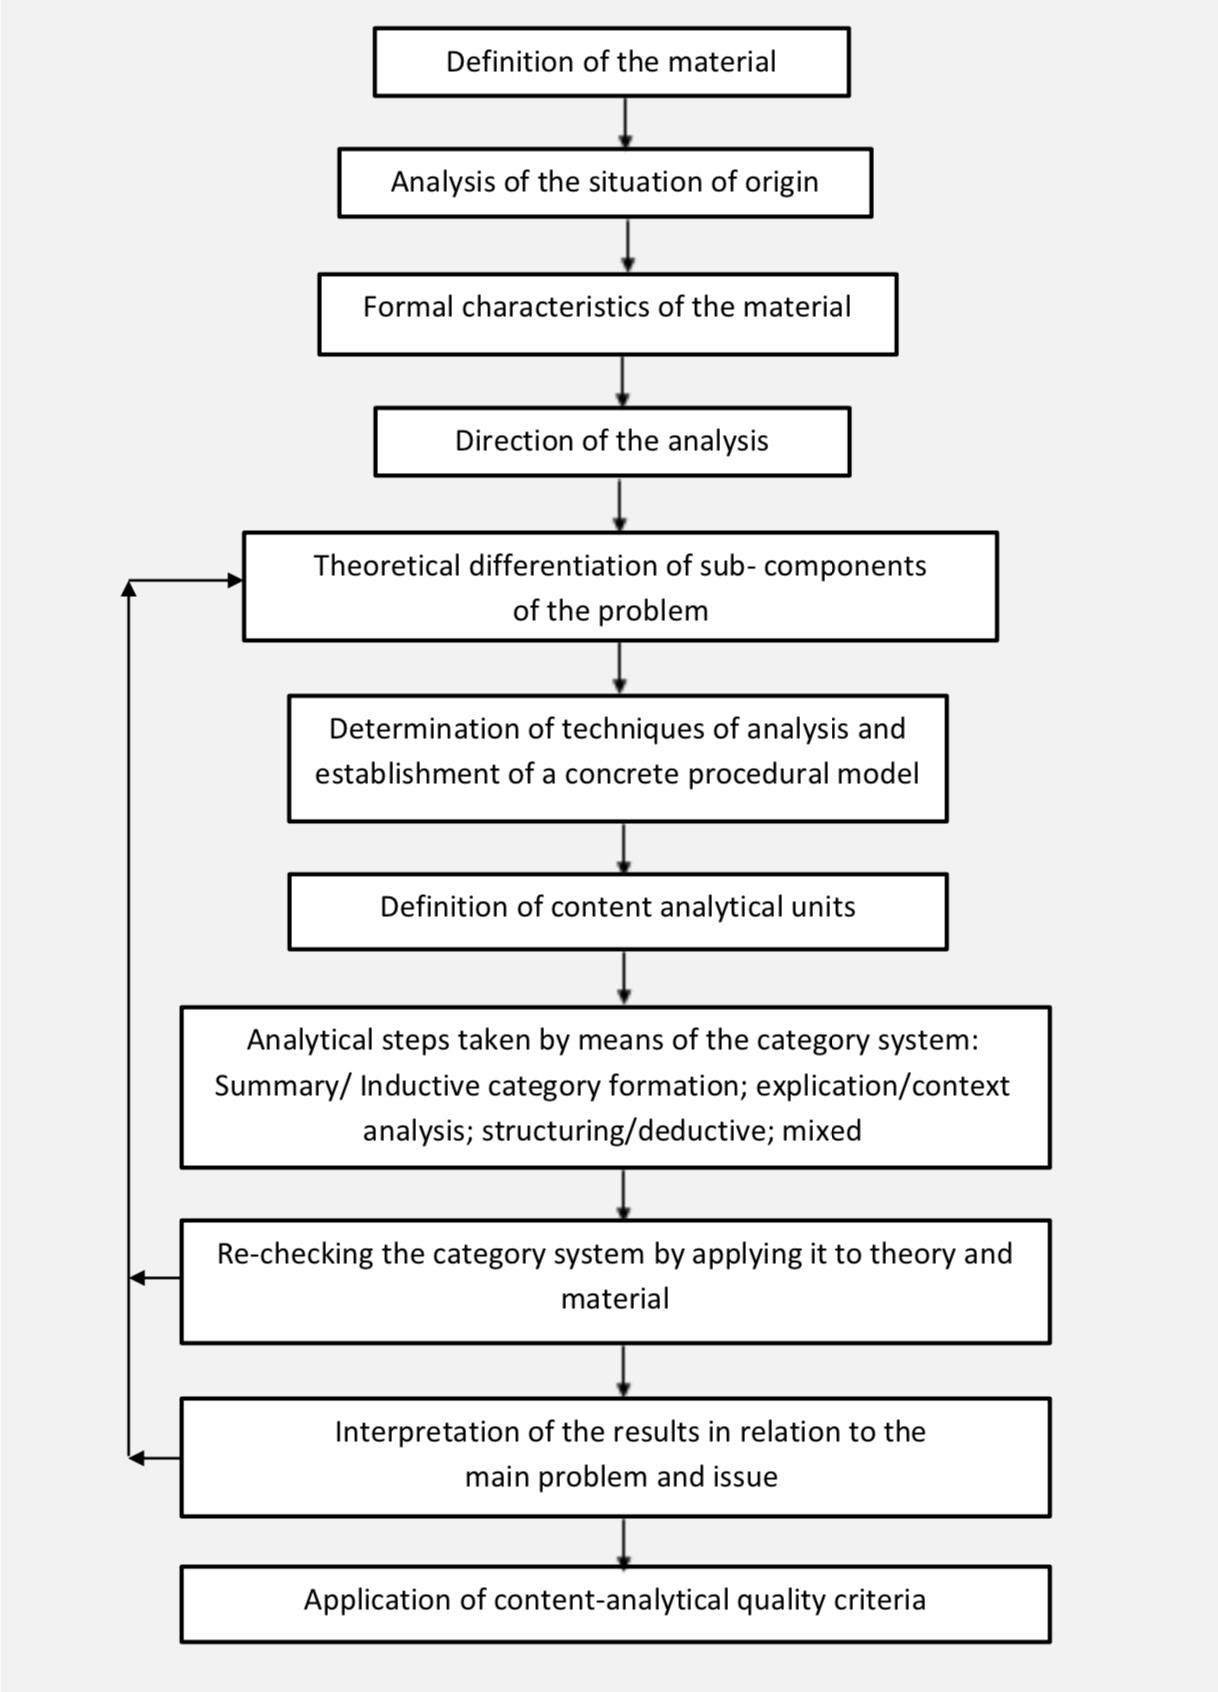
\includegraphics[width=0.8\textwidth]{graphics/MayringProcess.png}
    \caption[The general model of the content-analytical process.]{The general model of the content-analytical process.\footnotemark}
    \label{fig:MayringProcess}
\end{figure}
\footnotetext{Taken from \cite{MayringQualitativeContentAnalysis2014}, p.54}

This process is as a model and must be adapted to fit the material and the specific research problem. For this study, the purpose of the analysis is to extract information regarding the problems and struggles, the interviewees experience when trying to understand the blockchain technology. For this purpose, the material is summarized, which creates an abstraction from the material that correctly represents/generalized said material. \footcite[Cf.][p.68]{MayringQualitativeContentAnalysis2014} The summarizing technique is comprised of four steps: 1) Paraphrasing the content-bearing text components, 2) generalizing these to a certain abstraction level, 3) reducing these in a first attempt to remove semantically identical paraphrases and 4) reducing these a second time through binding and integration of paraphrases on the envisaged abstraction level. After these steps are completed, the new statements are put into the category system (step 8), whose exactness/applicability is tested after 10-50\% of material has been sighted. If the level of abstraction does not meet the desired level, the category system must be revised and all information re-evaluated.\footcite[Cf.][p.68 et seq]{MayringQualitativeContentAnalysis2014}

\anhangteil{The completed category system}

\textbf{Hier muss noch die Excel Tabelle irgendwie rein!}


\anhang{Screen clippings of the artifact}
\anhangteil{Overview, larger version of figure \ref{fig:OverviewPic}}

\begin{figure}[H]
    \centering
    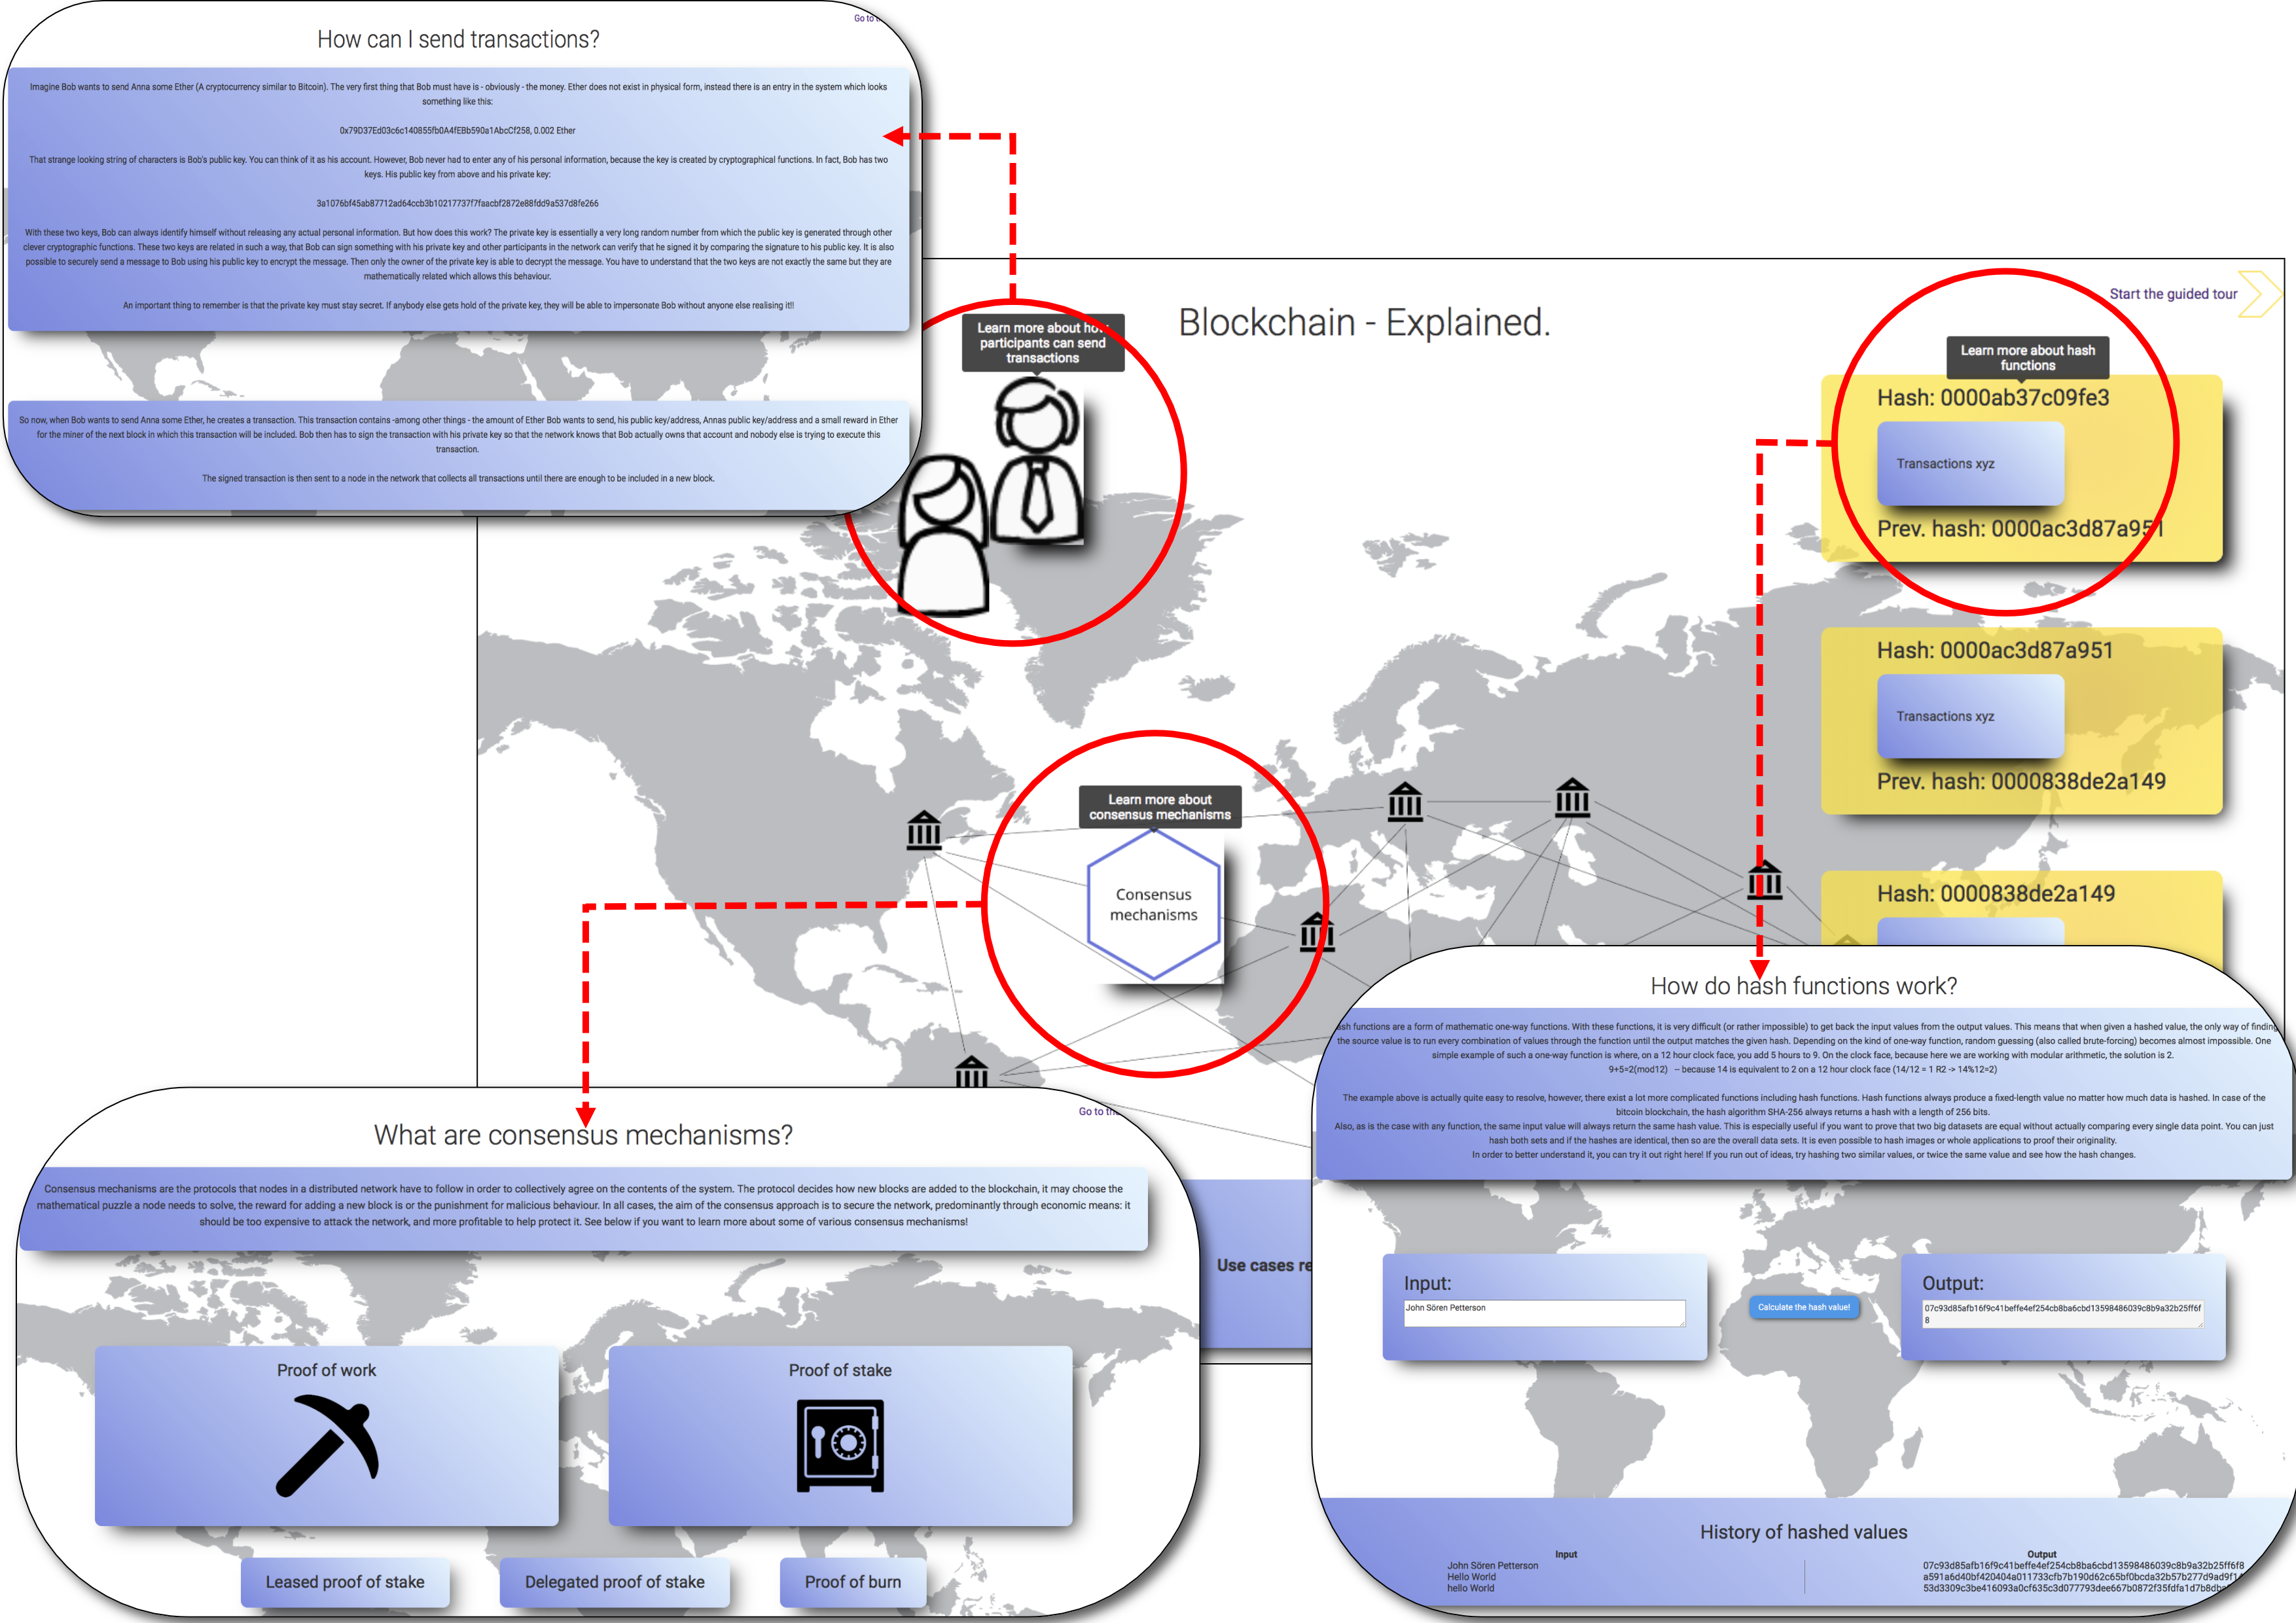
\includegraphics[height=0.9\textwidth, angle=90]{latex-vorlage_v1.5/graphics/Overview_Big.png}
    \caption{The symbols within the overview lead to more information regarding transactions, consensus mechanisms, hash functions and use cases (no red circle). Larger version of figure \ref{fig:OverviewPic}}
    \label{fig:my_label}
\end{figure}


\newpage 
\anhang{Evaluation assets}

\anhangteil{Questionnaire}\label{anhang:EvaluationQuestionnaire}

Before you watch the explanations or the tutorial, please respond to the following questions:
\begin{enumerate}
\newcounter{xy}
    \item Please answer the following questions with yes or no:
    \begin{enumerate}
        \item Do you know bitcoin?
        \item Do you understand how bitocin works?
        \item Do you know blockchain?
        \item Do you understand how blockchain works?
        \item Do you know what cryptoeconomics (the underlying concepts within finance, informatics, and economics) means?
    \end{enumerate}
    \item On a scale from 1 ("I do not know anything about it.") to 10 ("I understand the various different underlying components of the blockchain technology in detail."), how confident do you feel about your knowledge about blockchain technology?
    \item Please give a detailed response (roughly several sentences): How would you explain the blockchain technology to your peers?
    \item Please give a detailed response (roughly several sentences): Why and for what purpose would somebody want to use blockchain technology?
 \setcounter{xy}{\value{enumi}}
\end{enumerate}

Please answer the following questions after you have finished the videos or the tutorial:
\begin{enumerate}
\setcounter{enumi}{\value{xy}}
    \item Please answer the following questions with yes or no:
    \begin{enumerate}
        \item Do you know bitcoin?
        \item Do you understand how bitocin works?
        \item Do you know blockchain?
        \item Do you understand how blockchain works?
        \item Do you know what crypto economics (the underlying concepts within finance, informatics, and economics) means?
    \end{enumerate}
    \item On a scale from 1 ("I do not know anything about it.") to 10 ("I understand the various different underlying components of the blockchain technology in detail."), how confident do you feel about your knowledge about blockchain technology?
    \item Please give a detailed response (roughly several sentences): How would you explain the blockchain technology to your peers?
    \item Please give a detailed response (roughly several sentences): Why and for what purpose would somebody want to use blockchain technology?
    \item What did you like about the explanation?
    \item What did you dislike about the explanation? What elements were you missing?
\end{enumerate}

\anhangteil{Responses to the questionnaire} \label{anhang:ResponsesQuestionnaire}


